\begin{flushright} {\tiny {\color{gray} chapter4.tex}} \end{flushright}

\subsection{Numerical integration} \label{sec:quadrature}As we will see later, using the Finite Element method to solve problems involves computing integrals which are more often than not too complex to be computed analytically/exactly. We will then need to compute them numerically.

[wiki] In essence, 
the basic problem in numerical integration is to compute an approximate solution to a definite integral
\[
\int_a^b f(x) dx
\]
to a given degree of accuracy.
This problem has been widely studied and we know that 
if $f(x)$ is a smooth function, and the domain of integration is bounded, there are many methods for approximating the integral to the desired precision.

There are several reasons for carrying out numerical integration.
\begin{itemize}
\item The integrand $f(x)$ may be known only at certain points, such as obtained by sampling. Some embedded systems and other computer applications may need numerical integration for this reason.
\item A formula for the integrand may be known, but it may be difficult or impossible to find an antiderivative that is an elementary function. An example of such an integrand is $f(x)=exp(-x^2)$, the antiderivative of which (the error function, times a constant) cannot be written in elementary form.
\item It may be possible to find an antiderivative symbolically, but it may be easier to compute a numerical approximation than to compute the antiderivative. That may be the case if the antiderivative is given as an infinite series or product, or if its evaluation requires a special function that is not available.
\end{itemize}

%-----------------------------
\subsubsection{in 1D - theory}

The simplest method of this type is to let the interpolating function be a constant function (a polynomial of degree zero) that passes through the point $((a+b)/2, f((a+b)/2))$.

This is called the midpoint rule \index{midpoint rule} or rectangle rule. \index{rectangle rule}
\[
\int_a^b f(x)dx \simeq (b-a) f(\frac{a+b}{2})
\]

\improvement[inline]{insert here figure}

The interpolating function may be a straight line (an affine function, i.e. a polynomial of degree 1)
passing through the points $(a, f(a))$ and $(b, f(b))$.

This is called the trapezoidal rule. \index{trapezoidal rule} 
\[
\int_a^b f(x)dx \simeq (b-a) \frac{f(a)+f(b)}{2}
\]

\improvement[inline]{insert here figure}

For either one of these rules, we can make a more accurate approximation by breaking up the interval [a, b] into some number n of subintervals, computing an approximation for each subinterval, then adding up all the results. This is called a composite rule, extended rule, or iterated rule. For example, the composite trapezoidal rule can be stated as

\[
\int_a^b f(x)dx \simeq \frac{b-a}{n} \left( \frac{f(a)}{2}  
+\sum_{k=1}^{n-1} f(a+k\frac{b-a}{n})
   +\frac{f(b)}{2} \right)
\]

where the subintervals have the form $[kh,(k+1)h]$, with $h=(b-a)/n$ and $k=0,1,2,\dots,n-1$.


\begin{center}
a)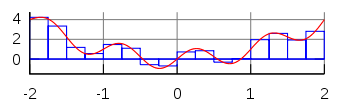
\includegraphics[width=7cm]{images/quadrature/int1}
b)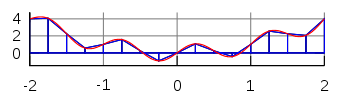
\includegraphics[width=7cm]{images/quadrature/int2}\\
The interval $[-2,2]$ is broken into 16 sub-intervals. The blue lines correspond to the 
approximation of the red curve by means of a) the midpoint rule,  b) the trapezoidal rule.
\end{center}

There are several algorithms for numerical integration (also commonly called 'numerical quadrature', or
simply 'quadrature') \index{quadrature}.
Interpolation with polynomials evaluated at equally spaced points in $[a,b]$
yields the Newton–Cotes formulas, of which the rectangle rule and the trapezoidal rule are examples. \index{Newton-Cotes}
If we allow the intervals between interpolation points to vary, we find another group of quadrature formulas, such as 
the Gauss(ian) quadrature formulas. \index{Gauss quadrature}
A Gaussian quadrature rule is typically more accurate than a Newton–Cotes rule, 
which requires the same number of function evaluations, if the integrand is smooth 
(i.e., if it is sufficiently differentiable).


An $n-$point Gaussian quadrature rule, named after Carl Friedrich Gauss, is a quadrature rule constructed
to yield an exact result for polynomials of degree $2n-1$ or less by a suitable choice of the points $x_i$
and weights $w_i$ for $i=1,\dots,n$.

The domain of integration for such a rule is conventionally taken as $[-1,1]$, so the rule is stated as
\[
\int_{-1}^{+1} f(x) dx = \sum_{i_q=1}^n w_{i_q} f(x_{i_q})
\]
In this formula the $x_{i_q}$ coordinate is 
the $i$-th root of the Legendre polynomial $P_n(x)$. \index{Legendre polynomial}

It is important to note that a Gaussian quadrature will only produce good results if the function $f(x)$
is well approximated by a polynomial function within the range $[-1,1]$.
As a consequence, the method is not, for example, suitable for functions with singularities.

\begin{center}
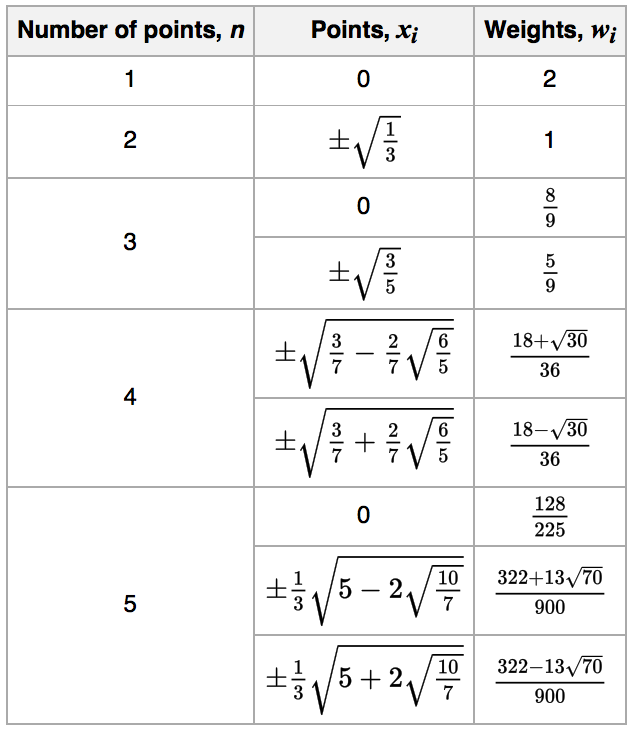
\includegraphics[width=5.cm]{images/quadrature/gq2}\\
Gauss-Legendre points and their weights.
\end{center}

\begin{tabular}{lllll}
\hline
n & $x_{iq}$ & $w_{iq}$ & $x_{iq}$ (approx) & $w_{iq}$ (approx) \\
\hline\hline
1 & 0 & 2 & 0 & 2 \\
\hline
2 & $\pm \sqrt{1/3}$ & 1  & $\pm$0.577350269189626 & 1 \\
\hline
3 & 0 & 8/9 & 0 & 0.888888888888889 \\
  & $\pm\sqrt{3/5}$  & 5/9  & $\pm$0.774596669241483 & 0.555555555555556 \\
\hline
4 & $\pm\sqrt{\frac{3}{7} - \frac{2}{7}\sqrt{6/5}}$  & $\frac{18+\sqrt{30}}{36}$ & $\pm$0.339981043584856 & 0.652145154862546 \\
  & $\pm\sqrt{\frac{3}{7} + \frac{2}{7}\sqrt{6/5}}$  & $\frac{18-\sqrt{30}}{36}$ & $\pm$0.861136311594053 & 0.347854845137454 \\
\hline
5 & 0 & 128/225 & 0 & 0.568888888888889 \\
  & $\pm\frac{1}{3}\sqrt{5-2\sqrt{\frac{10}{7}}}$  & $\frac{322+13\sqrt{70}}{900}$ & $\pm$0.538469310105683 & 0.478628670499366 \\
  & $\pm\frac{1}{3}\sqrt{5+2\sqrt{\frac{10}{7}}}$  & $\frac{322-13\sqrt{70}}{900}$ & $\pm$0.906179845938664 & 0.236926885056189 \\
\hline
6 & ?& ?& $\pm$0.23861 91860 83197 & 0.46791 39345 72691 \\
  & ?& ?& $\pm$0.66120 93864 66265 & 0.36076 15730 48139 \\
  & ?& ?& $\pm$0.93246 95142 03152 & 0.17132 44923 79170 \\
\hline
\end{tabular}



As shown in the above table, it can be shown that the weight values must fulfill the following condition:
\begin{equation}
\sum_{i_q} w_{i_q}=2 \label{gq23}
\end{equation}
and it is worth noting that all quadrature point coordinates are symmetrical around the origin.

Since most quadrature formula are only valid on a specific interval, we now must address the problem 
of their use outside of such intervals. The solution turns out to be quite simple: one 
must carry out a change of variables from the interval $[a,b]$ to $[-1,1]$.

We then consider the reduced coordinate $r\in[-1,1]$ such that 
\[
r=\frac{2}{b-a}(x-a)-1 
\]
This relationship can be reversed such that when $r$ is known, its equivalent coordinate 
$x\in[a,b]$ can be computed:
\[
x=\frac{b-a}{2}(1+r)+a
\]
From this it follows that
\[
dx=\frac{b-a}{2}dr
\]
and then 
\[
\int_a^b f(x) dx  = \frac{b-a}{2} \int_{-1}^{+1} f(r) dr \simeq 
\frac{b-a}{2} \sum_{i_q=1}^n w_{i_q} f(r_{i_q})
\]

%--------------------
\subsubsection{in 1D - examples}

\paragraph{example 1}

Since we know how to carry out any required change of variables, we choose for simplicity 
$a=-1$, $b=+1$.
Let us take for example $f(x)=\pi$. Then we can compute the integral of this function 
over the interval $[a,b]$ exactly:
\[
I=\int_{-1}^{+1} f(x) dx = \pi \int_{-1}^{+1}dx  = 2 \pi
\]
We can now use a Gauss-Legendre formula to compute this same integral:
\[
I_{gq}=\int_{-1}^{+1} f(x) dx 
= \sum_{i_q=1}^{n_q} w_{i_q} f(x_{i_q}) 
= \sum_{i_q=1}^{n_q} w_{i_q} \pi
= \pi \underbrace{\sum_{i_q=1}^{n_q} w_{i_q} }_{=2}
= 2 \pi
\]
where we have used the property of the weight values of Eq.(\ref{gq23}).
Since the actual number of points was never specified, this result is valid for all 
quadrature rules.


\paragraph{example 2}

Let us now take $f(x)=m x+ p$ and repeat the same exercise:
\[
I=\int_{-1}^{+1} f(x) dx = \int_{-1}^{+1} (mx+p) dx  =  [\frac{1}{2} m x^2 + p x ]_{-1}^{+1} =2p
\]
\[
I_{gq}=\int_{-1}^{+1} f(x) dx 
\!= \sum_{i_q=1}^{n_q} w_{i_q} f(x_{i_q}) 
\!= \sum_{i_q=1}^{n_q} w_{i_q} (m x_{i_q} + p)  
\!= m \underbrace{\sum_{i_q=1}^{n_q} w_{i_q} x_{i_q}}_{=0}  + p \underbrace{\sum_{i_q=1}^{n_q} w_{i_q}}_{=2}  = 2p
\]
since the quadrature points are symmetric w.r.t. to zero on the x-axis.
Once again the quadrature is able to compute the exact value of this integral: this makes sense since 
an $n$-point rule exactly integrates a $2n-1$ order polynomial such that a 1 point quadrature exactly 
integrates a first order polynomial like the one above.



\paragraph{example 3}

Let us now take $f(x)=x^2$. We have 
\[
I=\int_{-1}^{+1} f(x) dx = \int_{-1}^{+1} x^2 dx  =  [\frac{1}{3}x^3 ]_{-1}^{+1} =  \frac{2}{3} 
\]
and 
\[
I_{gq}=\int_{-1}^{+1} f(x) dx 
\!= \sum_{i_q=1}^{n_q} w_{i_q} f(x_{i_q}) 
\!= \sum_{i_q=1}^{n_q} w_{i_q} x_{i_q}^2 
\]

\begin{itemize}
\item $n_q=1$: $x_{iq}^{(1)}=0$, $w_{i_q}=2$. $I_{gq}=0$
\item $n_q=2$: $x_{q}^{(1)}=-1/\sqrt{3}$, $x_{q}^{(2)}=1/\sqrt{3}$, $w_{q}^{(1)}=w_{q}^{(2)}=1$. $I_{gq}=\frac{2}{3}$
\item It also works $\forall n_q>2$ !
\end{itemize}

%-----------------------------
\subsubsection{in 2D/3D - theory}


Let us now turn to a two-dimensional integral of the form
\[
I=\int_{-1}^{+1} \int_{-1}^{+1} f(x,y) dx dy
\]
The equivalent Gaussian quadrature writes:
\[
I_{gq}
\simeq \sum_{i_q=1}^{n_q}\sum_{j_q}^{n_q} f(x_{i_q},y_{j_q}) w_{i_q} w_{j_q}
\]

%----------------------------------------
\subsubsection{quadrature on triangles}

Quadrature rules for triangles can be found in Dunavant, 1985 \cite{duna85}.
The following ones are identical to those in the {\sl ip\_triangle.m} 
file of the MILAMIN code \cite{daks08}.

{\small
\[
\begin{array}{ccccccc}
\hline
&r_q & s_q & w_q \\ 
\hline\hline
iq=1& 1/3 & 1/3 & 1/2\\
\hline
iq=1 & 1/6 & 1/6 & 1/6 \\
iq=2 & 2/3 & 1/6 & 1/6 \\
iq=3 & 1/6 & 2/3 & 1/6 \\
\hline
iq=1&1/3 & 1/3 & -27/96\\
iq=2&0.6 & 0.2 &  25/96\\
iq=3&0.2 & 0.6 &  25/96\\
iq=4&0.2 & 0.2 &  25/96\\
\hline
iq=1& 1-2g_1 & g_1 & w_1/2  &  0.108103018168070 & 0.44594849091596  &   \\
iq=2& g_1 & 1-2g_1 & w_1/2  &  0.445948490915965 & 0.108103018168070 &   \\
iq=3& g_1 & g_1    & w_1/2  &  0.445948490915965 & 0.445948490915965 &   \\
iq=4& 1-2g_2 & g_2 & w_2/2  &  0.816847572980459 & 0.091576213509771 &   \\
iq=5& g_2 & 1-2g_2 & w_2/2  &  0.091576213509771 & 0.816847572980459 &   \\
iq=6& g_2 & g_2    & w_2/2  &  0.091576213509771 & 0.091576213509771 &   \\
\hline
iq=1&&&&0.091576213509771 &  0.091576213509771    &    0.109951743655322/2.0 \\ 
iq=2&&&&0.816847572980459 &  0.091576213509771    &    0.109951743655322/2.0 \\
iq=3&&&&0.091576213509771 &  0.816847572980459    &    0.109951743655322/2.0 \\
iq=4&&&&0.445948490915965 &  0.445948490915965    &    0.223381589678011/2.0 \\
iq=5&&&&0.108103018168070 &  0.445948490915965    &    0.223381589678011/2.0 \\
iq=6&&&&0.445948490915965 &  0.108103018168070    &    0.223381589678011/2.0 \\
\hline
iq=1 &&&&0.1012865073235 &  0.1012865073235  &     0.0629695902724 \\
iq=2 &&&&0.7974269853531 &  0.1012865073235  &     0.0629695902724 \\
iq=3 &&&&0.1012865073235 &  0.7974269853531  &     0.0629695902724 \\
iq=4 &&&&0.4701420641051 &  0.0597158717898  &     0.0661970763942 \\
iq=5 &&&&0.4701420641051 &  0.4701420641051  &     0.0661970763942 \\
iq=6 &&&&0.0597158717898 &  0.4701420641051  &     0.0661970763942 \\
iq=7 &&&&0.3333333333333 &  0.3333333333333  &     0.1125000000000 \\
\hline
iq=1&&&& 5.01426509658179E-01&  2.49286745170910E-01 &   5.83931378631895E-02 \\ 
iq=2&&&& 2.49286745170910E-01&  5.01426509658179E-01 &   5.83931378631895E-02 \\ 
iq=3&&&& 2.49286745170910E-01&  2.49286745170910E-01 &   5.83931378631895E-02 \\ 
iq=4&&&& 8.73821971016996E-01&  6.30890144915020E-02 &   2.54224531851035E-02 \\ 
iq=5&&&& 6.30890144915020E-02&  8.73821971016996E-01 &   2.54224531851035E-02 \\ 
iq=6&&&& 6.30890144915020E-02&  6.30890144915020E-02 &   2.54224531851035E-02 \\ 
iq=7&&&& 5.31450498448170E-02&  3.10352451033784E-01 &   4.14255378091870E-02 \\ 
iq=8&&&& 6.36502499121399E-01&  5.31450498448170E-02 &   4.14255378091870E-02 \\ 
iq=9&&&& 3.10352451033784E-01&  6.36502499121399E-01 &   4.14255378091870E-02 \\ 
iq=10&&&& 5.31450498448170E-02&  6.36502499121399E-01 &   4.14255378091870E-02 \\ 
iq=11&&&& 6.36502499121399E-01&  3.10352451033784E-01 &   4.14255378091870E-02 \\ 
iq=12&&&& 3.10352451033784E-01&  5.31450498448170E-02 &   4.14255378091870E-02 \\ 
\hline
\end{array}
\]
}

where
\[ 
g_1 = \left(8-\sqrt{10} + \sqrt{38-44\sqrt{2/5}}\right)/18
\qquad
g_2 = \left(8-\sqrt{10} - \sqrt{38-44\sqrt{2/5}}\right)/18
\]
\[
w_1 = \left(620+\sqrt{213125-53320\sqrt{10}}\right)/3720
\qquad
w_2 = \left(620-\sqrt{213125-53320\sqrt{10}}\right)/3720
\]


      


%----------------------------------------
\subsubsection{quadrature on tetrahedra}

\begin{remark}
In what follows the coefficients in the tables are not the reduced coordinates
of the quadratue points but the coefficients corresponding to the 4 nodes.
\end{remark}

Quadrature rules on tetrahedra take the form:
\[
\int\int\int_{el} f(x,y,z) dxdydz = V_{el} \sum_{iq=1}^{nqel} w_{iq} f(\xi^{iq}_1,\xi^{iq}_2,\xi^{iq}_3,\xi^{iq}_4) 
\]
or, that is to say:
\[
\int\int\int_{el} f(x,y,z) dxdydz = \sum_{iq=1}^{nqel} (w_{iq}V_{el}) f(\xi^{iq}_1,\xi^{iq}_2,\xi^{iq}_3,\xi^{iq}_4) 
\]
with in our case $V_{el}=1/6$.

In the literature it can be found that a one point quadrature is characterised by 
\[
w_{iq}=1 \quad\quad\quad \xi^{iq}_1=\xi^{iq}_2=\xi^{iq}_3=\xi^{iq}_4=0.25
\]
i.e, the coordinates of the single point are given by:
\[
x_{iq}=\sum_{i=1}^4 \xi_i^{iq} x_i = \frac{1}{4} (x_1+x_2+x_3+x_4)
\]
Same for $y$ and $z$ coordinates. 

A four-point quadrature rule is characterised by $w_{iq}=V_el*0.25=1/24\simeq 04166666666666667$ and 

\begin{tabular}{lcccc}
 & $\xi_1$ & $\xi_2$ & $\xi_3$ & $\xi_4$ \\
iq=1 & 0.585410196624969 & 0.138196601125011 & 0.138196601125011 & 0.138196601125011 \\
iq=2 & 0.138196601125011 & 0.585410196624969 & 0.138196601125011 & 0.138196601125011 \\
iq=3 & 0.138196601125011 & 0.138196601125011 & 0.585410196624969 & 0.138196601125011 \\
iq=4 & 0.138196601125011 & 0.138196601125011 & 0.138196601125011 & 0.585410196624969 \\
\end{tabular}

We then have:
\[
r_{iq}=\sum_{i=1}^4 \xi_i^{iq} x_i 
= (\xi_1^{iq},\xi_2^{iq},\xi_3^{iq},\xi_4^{iq})\cdot(r_1,r_2,r_3,r_4) 
= (\xi_1^{iq},\xi_2^{iq},\xi_3^{iq},\xi_4^{iq})\cdot(0,1,0,0) 
= \xi_2^{iq}
\]
\[
s_{iq}=\sum_{i=1}^4 \xi_i^{iq} y_i 
= (\xi_1^{iq},\xi_2^{iq},\xi_3^{iq},\xi_4^{iq})\cdot(s_1,s_2,s_3,s_4) 
= (\xi_1^{iq},\xi_2^{iq},\xi_3^{iq},\xi_4^{iq})\cdot(0,0,1,0) 
= \xi_3^{iq}
\]
\[
t_{iq}=\sum_{i=1}^4 \xi_i^{iq} z_i 
= (\xi_1^{iq},\xi_2^{iq},\xi_3^{iq},\xi_4^{iq})\cdot(t_1,t_2,t_3,t_4) 
= (\xi_1^{iq},\xi_2^{iq},\xi_3^{iq},\xi_4^{iq})\cdot(0,0,0,1) 
= \xi_4^{iq}
\]
Finally:

\[
\begin{array}{ccccc}
     & r_q & s_q & t_q  & w_q \\
iq=1 & 0.138196601125011 & 0.138196601125011 & 0.138196601125011 & 0.04166666666666667\\
iq=2 & 0.585410196624969 & 0.138196601125011 & 0.138196601125011 & 0.04166666666666667\\
iq=3 & 0.138196601125011 & 0.585410196624969 & 0.138196601125011 & 0.04166666666666667\\
iq=4 & 0.138196601125011 & 0.138196601125011 & 0.585410196624969 & 0.04166666666666667\\
\end{array}
\]




 %----------------------
\newpage
\subsection{A bit of FE terminology} 
We introduce here some terminology for efficient element descriptions \cite{grsa}:
\begin{itemize}
\item For triangles/tetrahedra, the designation 
$P_m \times P_n$ \index{$P_m \times P_n$}
means that each component of the velocity
is approximated by continuous piecewise \index{piecewise} complete Polynomials of degree $m$ and
pressure by continuous piecewise complete Polynomials of degree  $n$.
For example $P_2 \times P_1$ means 
\[
u \sim a_1 + a_2 x + a_3 y + a_4 xy + a_5 x^2 + a_6 y^2
\]
with similar approximations for $v$, and 
\[
p \sim b_1 + b_2x + b_3 y
\]
Both velocity and pressure are continuous across element boundaries, 
and each triangular element contains 6 velocity nodes and three pressure nodes.

\item For the same families, \index{$P_m \times P_{-n}$} 
$P_m \times P_{-n}$
is as above, except that pressure is approximated via 
piecewise {\sl discontinuous} polynomials of degree $n$. For instance, $P_2 \times P_{-1}$ is the same 
as $P_2P_1$ except that pressure is now an independent linear function in each element and therefore 
discontinuous at element boundaries.

\item For quadrilaterals/hexahedra, the designation 
\index{$Q_m \times Q_n$}  $Q_m \times Q_n$
means that each component of the velocity
is approximated by a continuous piecewise polynomial of degree $m$ {\sl in each direction} on the quadrilateral
and likewise for pressure, except that the polynomial is of degree $n$.
For instance,  $Q_2 \times Q_1$ \index{$Q_2 \times Q_1$} means
\[
u \sim a_1 + a_2 x + a_3 y + a_4 xy + a_5 x^2 + a_6 y^2 + a_7 x^2y + a_8 xy^2 + a_9 x^2y^2
\]
and 
\[
p \sim b_1 + b_2x + b_3 y + b_4 xy
\]
\item For these same families, $Q_m \times Q_{-n}$ is as above, except that the pressure approximation 
is not continuous at element boundaries. \index{$Q_m \times Q_{-n}$}

\item Again for the same families, \index{$Q_m \times P_{-n}$} $Q_m \times P_{-n}$
 indicates the same velocity approximation 
with a pressure approximation that is a discontinuous complete piecewise polynomial of degree $n$
(not of degree $n$ in each direction !)

\item The designation $P_m^+$ or $Q_m^+$ means that some sort of bubble function \index{bubble function}
was added to the polynomial approximation for the velocity. You may also find the term 'enriched element'
in the literature.

\item Finally, for $n=0$, we have piecewise-constant pressure, and we omit the minus sign for simplicity.
\end{itemize}

Another point which needs to be clarified is the use of so-called 'conforming elements' 
(or 'non-conforming elements'). \index{conforming element} \index{non-conforming element}
Following again \cite{grsa}, conforming velocity elements are those for which the basis functions for a subset 
of $H^1$ for the continuous problem (the first derivatives and their squares are integrable in $\Omega$).
For instance, the rotated $Q_1 \times P_0$ element of Rannacher and Turek (see section \ref{ncq1p0}) is such that 
the velocity is discontinous across element edges, so that the derivative does not exist there. Another
typical example of non-conforming element is the Crouzeix-Raviart element \cite{crra73}.

 


 %-----------------------------------------
\newpage
\subsection{Elements and basis functions in 1D}\label{sec:elts1D} 
%------------------------------------------
\subsubsection{Linear basis functions ($Q_1$)}
\index{$Q_1$}

Let $f(r)$ be a $C^1$ function on the interval $[-1:1]$ with $f(-1)=f_1$  and $f(1)=f_2$.
\begin{center}
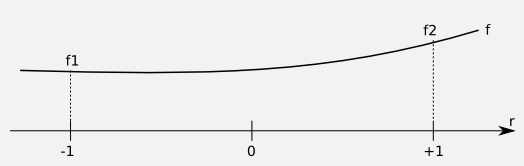
\includegraphics[width=8cm]{images/linshapefct.png}
\end{center}
Let us assume that the function $f(r)$ is to be approximated on $[-1,1]$ by the first order polynomial 
\begin{equation}
f(r)=a+br \label{eqquad1}
\end{equation}
Then it must fulfill
\begin{eqnarray}
f(r=-1)&=&a-b =f_1 \nonumber\\
f(r=+1)&=&a+b =f_2 \nonumber
\end{eqnarray}
This leads to  
\[
a=\frac{1}{2}(f_1+f_2)  
\quad\quad
b=\frac{1}{2}(-f_1+f_2)  
\]
and then replacing $a,b$ in Eq. (\ref{eqquad1}) by the above values on gets
\[
f(r) = \left[  \frac{1}{2}(1-r)\right] f_1 + \left[ \frac{1}{2}(1+r) \right] f_2
\]
or
\[
f(r)=\sum_{i=1}^2 N_i(r) f_1
\]
with
\begin{mdframed}[backgroundcolor=blue!5]
\begin{eqnarray}
N_1(r) &=& \frac{1}{2} (1-r) \nonumber\\
N_2(r) &=& \frac{1}{2} (1+r)
\end{eqnarray}
\end{mdframed}

%------------------------------------------
\subsubsection{Quadratic basis functions ($Q_2$)}
\index{$Q_2$}

Let $f(r)$ be a $C^1$ function on the interval $[-1:1]$ with $f(-1)=f_1$, $f(0)=f_2$ and $f(1)=f_3$.
\begin{center}
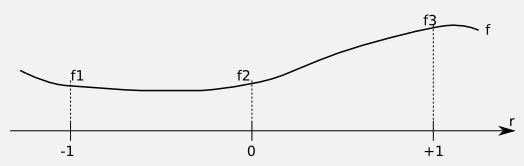
\includegraphics[width=8cm]{images/quadshapefct.png}
\end{center}

Let us assume that the function $f(r)$ is to be approximated on $[-1,1]$ by the second order polynomial
\begin{equation}
f(r)=a+br+cr^2 \label{eqquad}
\end{equation}
Then it must fulfill
\begin{eqnarray}
f(r=-1)&=&a-b+c = f_1 \nonumber\\
f(r=0) &=&a\quad\quad\quad\;     = f_2 \nonumber\\
f(r=+1)&=&a+b+c = f_3 \nonumber
\end{eqnarray}
This leads to
\[
a=f_2 
\quad
b=\frac{1}{2}(-f1+f3)
\quad
c=\frac{1}{2}(f_1+f_3-2f_2)
\]
and then replacing $a,b,c$ in Eq. (\ref{eqquad}) by the above values on gets
\[
f(r)=\left[\frac{1}{2}r(r-1)\right] f_1 + (1-r^2) f_2 + \left[\frac{1}{2}r(r+1)\right] f_3
\]
or,
\[
f(r) = \sum_{i=1}^3 N_i(r) f_i
\]
with
\begin{mdframed}[backgroundcolor=blue!5]
\begin{eqnarray}
N_1(r) &=& \frac{1}{2}r(r-1) \nonumber\\
N_2(r) &=& (1-r^2) \nonumber\\ 
N_3(r) &=& \frac{1}{2}r(r+1) 
\end{eqnarray}
\end{mdframed}



%------------------------------------------
\subsubsection{Cubic basis functions ($Q_3$)}
\index{$Q_3$}

The 1D basis polynomial is given by
\[
f(r)=a+br+cr^2+dr^3
\]
with the nodes at position -1,-1/3, +1/3 and +1.

\begin{eqnarray}
f(-1)   &=& a-b+c-d = f_1 \nonumber\\
f(-1/3) &=& a-\frac{b}{3}+\frac{c}{9}-\frac{d}{27} = f_2 \nonumber\\
f(+1/3) &=& a-\frac{b}{3}+\frac{c}{9}-\frac{d}{27} = f_3 \nonumber\\
f(+1)   &=& a+b+c+d = f_4 \nonumber
\end{eqnarray}

Adding the first and fourth equation and the second and third, one arrives at
\[
f_1+f_4 = 2a+2c \quad\quad\quad f_2+f_3=2a+\frac{2c}{9}
\]
and finally:
\[
a=\frac{1}{16} \left( -f_1 + 9f_2 + 9f_3 - f_4  \right)
\]
\[
c=\frac{9}{16}\left(f_1-f_2-f_3+f_4\right)
\]
Combining the original 4 equations in a different way yields
\[
2b+2d=f_4-f_1 
\quad\quad\quad
\frac{2b}{3} + \frac{2d}{27} = f_3-f_2
\]
so that
\[
b=\frac{1}{16} \left( f_1 - 27f_2 + 27f_3 -f_4   \right)
\]
\[
d=\frac{9}{16} \left( -f_1 + 3f_2 - 3f_3 + f_4 \right)
\]
Finally,

\begin{eqnarray}
f(r) 
&=& a+b+cr^2+dr^3 \nonumber\\
&=& \frac{1}{16} (-1+  r +9r^2 - 9r^3 )f_1 \nonumber\\ 
&+& \frac{1}{16} ( 9-27r -9r^2 +27r^3 )f_2 \nonumber\\ 
&+& \frac{1}{16} ( 9+27r -9r^2 -27r^3 )f_3 \nonumber\\ 
&+& \frac{1}{16} (-1-  r +9r^2 + 9r^3 )f_4 \nonumber\\ 
&=& \sum_{i=1}^4 N_i(r) f_i \nonumber
\end{eqnarray}
where
\begin{mdframed}[backgroundcolor=blue!5]
\begin{eqnarray}
N_1&=& \frac{1}{16} (-1+  r+9r^2- 9r^3 ) \nonumber\\ 
N_2&=& \frac{1}{16} ( 9-27r-9r^2+27r^3 ) \nonumber\\ 
N_3&=& \frac{1}{16} ( 9+27r-9r^2-27r^3 ) \nonumber\\ 
N_4&=& \frac{1}{16} (-1-  r+9r^2+ 9r^3 ) \nonumber
\end{eqnarray}
\end{mdframed}
Verification:

\begin{itemize}
\item
Let us assume $f(r)=C$, then
\[
\hat{f}(r) = \sum N_i(r) f_i = \sum_i N_i C = C \sum_i N_i  = C
\]
so that a constant function is exactly reproduced, as expected.

\item
Let us assume $f(r)= r$, then $f_1=-1$, $f_2=-1/3$, $f_3=1/3$ and $f_4=+1$. We then have
\begin{eqnarray}
\hat{f}(r) 
&=& \sum N_i(r) f_i  \nonumber\\
&=& - N_1(r) -\frac{1}{3}N_2(r) + \frac{1}{3}N_3(r)  + N_4(r) \nonumber\\
&=& [-(-1+  r+9r^2- 9r^3 ) \nn\\
&&- \frac{1}{3} ( 9-27r-9r^2-27r^3 ) \nn\\
&&+ \frac{1}{3} ( 9+27r-9r^2+27r^3 ) \nn\\
&&+ (-1-  r+9r^2+ 9r^3 )]/16 \nonumber\\
&=& [-r +9r + 9r -r]/16  + ... 0 ... \nonumber\\
&=& r   
\end{eqnarray}

\end{itemize}


The basis functions derivative are given by
\begin{mdframed}[backgroundcolor=blue!5]
\begin{eqnarray}
 \frac{\partial N_1}{\partial r}&=& \frac{1}{16}  (  1 +18r - 27r^2 ) \nonumber\\ 
 \frac{\partial N_2}{\partial r}&=& \frac{1}{16}  (-27 -18r + 81r^2 ) \nonumber\\ 
 \frac{\partial N_3}{\partial r}&=& \frac{1}{16}  (+27 -18r - 81r^2 ) \nonumber\\ 
 \frac{\partial N_4}{\partial r}&=& \frac{1}{16}  ( -1 +18r + 27r^2 ) \nonumber
\end{eqnarray}
\end{mdframed}
Verification:

\begin{itemize}
\item
Let us assume $f(r)=C$, then
\begin{eqnarray}
\frac{\partial \hat{f}}{\partial r} 
&=& \sum_i \frac{\partial N_i}{\partial r} f_i  \nonumber\\
&=&  C \sum_i \frac{\partial N_i}{\partial r}  \nonumber\\
&=& \frac{C}{16} [  (  1 +18r - 27r^2 ) \nn\\
&&+ (-27 -18r + 81r^2 )  \nn\\
&&+  (+27 -18r - 81r^2 ) \nn\\
&&+ ( -1 +18r + 27r^2 ) ]  \nonumber\\
&=& 0 \nonumber
\end{eqnarray}

\item
Let us assume $f(r)= r$, then $f_1=-1$, $f_2=-1/3$, $f_3=1/3$ and $f_4=+1$. We then have
\begin{eqnarray}
\frac{\partial \hat{f}}{\partial r} 
&=& \sum_i \frac{\partial N_i}{\partial r} f_i  \nonumber\\
&=& \frac{1}{16} [  -(  1 +18r - 27r^2 ) \nn\\ 
&& -\frac{1}{3} (-27 -18r + 81r^2 )  \nn\\
&& +\frac{1}{3}  (+27 -18r - 81r^2 ) \nn\\
&& + ( -1 +18r + 27r^2 ) ]  \nonumber\\
&=& \frac{1}{16} [-2 + 18 + 54r^2 - 54r^2] \nonumber\\
&=& 1 \nonumber
\end{eqnarray}

\end{itemize}


 %-------------
\newpage
\subsection{Elements and basis functions in 2D}\label{sec:shpfct2d} Let us for a moment consider a single quadrilateral element in the $xy$-plane, 
as shown on the following figure:
\begin{center}
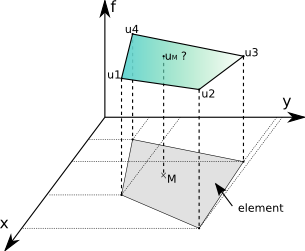
\includegraphics[width=5.8cm]{images/shape.png}
\end{center}
Let us assume that we know the values of a given field $u$ at the vertices.
For a given point $M$ inside the element in the plane, what is the value of the 
field $u$ at this point?
It makes sense to postulate that $u_M=u(x_M,y_M)$ will be given  by 
\[
u_M= \phi(u_1,u_2,u_3,u_4,x_M,y_M) 
\]
where $\phi$ is a function to be determined. Although $\phi$ is not unique, we can 
decide to express the value $u_M$ as a weighed sum of the values at the vertices $u_i$.
One option could be to assign all four vertices the same weight, say $1/4$ so that 
$u_M=(u_1+u_2+u_3+u_4)/4$, i.e. $u_M$ is simply given by the arithmetic mean 
of the vertices values. This approach suffers from a major drawback as it does
not use the location of point $M$ inside the element. For instance, when 
$(x_M,y_M) \rightarrow (x_2,y_2)$ we expect $u_M \rightarrow u_2$.

In light of this, we could now assume that the weights would depend on the position 
of $M$ in a continuous fashion:
\[
u(x_M,y_M) = \sum_{i=1}^4 N_i(x_M,y_M)\;  u_i
\]
where the $N_i$ are continous ("well behaved") functions which have the property:
\[
N_i(x_j,y_j)=\delta_{ij}
\]
or, in other words: 
\begin{eqnarray}
N_3(x_1,y_1) &=& 0 \\
N_3(x_2,y_2) &=& 0 \\
N_3(x_3,y_3) &=& 1 \\
N_3(x_4,y_4) &=& 0 
\end{eqnarray}
The functions $N_i$ are commonly called basis functions. \index{basis functions}

Omitting the $M$ subscripts for any point inside the element, the velocity components $u$
and $v$ are given by:
\begin{eqnarray}
\hat{u}(x,y) &=& \sum_{i=1}^4 N_i(x,y)\;  u_i \\
\hat{v}(x,y) &=& \sum_{i=1}^4 N_i(x,y)\;  v_i \label{bf01}
\end{eqnarray}
Rather interestingly, one can now easily compute velocity gradients (and therefore the 
strain rate tensor) since we have assumed the basis functions to be "well behaved" 
(in this case differentiable):
\begin{eqnarray}
\dot{\epsilon}_{xx}(x,y) &=& \frac{\partial u}{\partial x} = \sum_{i=1}^4 \frac{\partial N_i}{\partial x}\;  u_i \\
\dot{\epsilon}_{yy}(x,y) &=& \frac{\partial v}{\partial y} = \sum_{i=1}^4 \frac{\partial N_i}{\partial y}\;  v_i \\
\dot{\epsilon}_{xy}(x,y) &=& \frac{1}{2}\frac{\partial u}{\partial y} 
+ \frac{1}{2}\frac{\partial v}{\partial x} 
= \frac{1}{2}\sum_{i=1}^4 \frac{\partial N_i}{\partial y}\;  u_i
+ \frac{1}{2}\sum_{i=1}^4 \frac{\partial N_i}{\partial x}\;  v_i
\end{eqnarray}
How we actually obtain the exact form of the basis functions is explained in the coming section.










%%%%%%%%%%%%%%%%%%%%%%%%%%%%%%%%%%%%%%%%%%%%%%%%%%%%%%%
\subsubsection{Bilinear basis functions in 2D ($Q_1$)}
\index{$Q_1$}

In this section, we place ourselves in the most favorables case, i.e. the element is a square defined 
by $-1<r<1$, $-1<s<1$ in the Cartesian coordinates system $(r,s)$:

\begin{verbatim}
3===========2       
|           |     (r_0,s_0)=(-1,-1)
|           |     (r_1,s_1)=(+1,-1)
|           |     (r_2,s_2)=(+1,+1)
|           |     (r_3,s_3)=(-1,+1)
|           |
0===========1
\end{verbatim}


This element is commonly called the reference element. How we go from the $(x,y)$ coordinate system 
to the $(r,s)$ once and vice versa will be dealt later on.
For now, the basis functions in the above reference element and in the reduced 
coordinates system $(r,s)$ are given by:

\begin{mdframed}[backgroundcolor=blue!5]
\begin{eqnarray}
N_1(r,s)&=&0.25(1-r)(1-s) \nonumber\\
N_2(r,s)&=&0.25(1+r)(1-s) \nonumber\\
N_3(r,s)&=&0.25(1+r)(1+s) \nonumber\\
N_4(r,s)&=&0.25(1-r)(1+s) \nonumber
\end{eqnarray}
\end{mdframed}

The partial derivatives of these functions with respect to $r$ ans $s$ automatically follow:

\begin{mdframed}[backgroundcolor=blue!5]
\begin{align}
\frac{\partial N_1}{\partial r}(r,s)&= - 0.25(1-s) &
\frac{\partial N_1}{\partial s}(r,s)&= - 0.25(1-r) \nonumber\\
\frac{\partial N_2}{\partial r}(r,s)&= + 0.25(1-s) &
\frac{\partial N_2}{\partial s}(r,s)&= - 0.25(1+r) \nonumber\\
\frac{\partial N_3}{\partial r}(r,s)&= + 0.25(1+s) &
\frac{\partial N_3}{\partial s}(r,s)&= + 0.25(1+r) \nonumber\\
\frac{\partial N_4}{\partial r}(r,s)&= - 0.25(1+s) &
\frac{\partial N_4}{\partial s}(r,s)&= + 0.25(1-r) \nonumber
\end{align}
\end{mdframed}

Let us go back to Eq.(\ref{bf01}). And let us assume that the function $v(r,s)=C$ so that $v_i=C$ for $i=1,2,3,4$. 
It then follows that 
\[
\hat{v}(r,s) = \sum_{i=1}^4 N_i(r,s)\;  v_i = C \sum_{i=1}^4 N_i(r,s)
=C [
N_1(r,s)
+N_2(r,s)
+N_3(r,s)
+N_4(r,s)]=C
\]
This is a very important property: if the $v$ function used to assign values at the vertices is constant, then 
the value of $\hat{v}$ {\it anywhere} in the element is exactly $C$.
If we now turn to the derivatives of $v$ with respect to $r$ and $s$:
\[
\frac{\partial \hat{v}}{\partial r}(r,s) = \sum_{i=1}^4 \frac{\partial N_i}{\partial r}(r,s)\;  v_i = C \sum_{i=1}^4 \frac{\partial N_i}{\partial r}(r,s) 
= C \left[ - 0.25(1-s)  + 0.25(1-s)  + 0.25(1+s)  - 0.25(1+s) \right] = 0 
\]

\[
\frac{\partial \hat{v}}{\partial s}(r,s) = \sum_{i=1}^4 \frac{\partial N_i}{\partial s}(r,s)\;  v_i = C \sum_{i=1}^4 \frac{\partial N_i}{\partial s}(r,s) 
= C \left[ - 0.25(1-r) - 0.25(1+r) + 0.25(1+r) + 0.25(1-r) \right] = 0 
\]
We reassuringly find that the derivative of a constant field anywhere in the element is exactly zero.

If we now choose $v(r,s)=ar+bs$ with $a$ and $b$ two constant scalars, we find:
\begin{eqnarray}
\hat{v}(r,s) 
&=& \sum_{i=1}^4 N_i(r,s)\;  v_i  \\
&=& \sum_{i=1}^4 N_i(r,s) (ar_i+bs_i) \\
&=& a \underbrace{\sum_{i=1}^4 N_i(r,s) r_i}_{r} + b \underbrace{\sum_{i=1}^4 N_i(r,s) s_i}_{s} \\
&=& a \left[ 
0.25(1-r)(1-s)(-1)
+0.25(1+r)(1-s)(+1)
+0.25(1+r)(1+s)(+1)
+0.25(1-r)(1+s)(-1) \right]  \nonumber\\
&+& b  
\left[ 
0.25(1-r)(1-s)(-1)
+0.25(1+r)(1-s)(-1)
+0.25(1+r)(1+s)(+1)
+0.25(1-r)(1+s)(+1) \right]  \nonumber\\
&=& a \left[ 
-0.25(1-r)(1-s)
+0.25(1+r)(1-s)
+0.25(1+r)(1+s)
-0.25(1-r)(1+s) \right]  \nonumber\\
&+& b  
\left[ 
-0.25(1-r)(1-s)
-0.25(1+r)(1-s)
+0.25(1+r)(1+s)
+0.25(1-r)(1+s) \right]  \nonumber\\
&=& ar+bs
\end{eqnarray}
{\color{red} verify above eq}.
This set of bilinear shape functions is therefore capable of exactly representing a bilinear field.
The derivatives are:
\begin{eqnarray}
\frac{\partial \hat{v}}{\partial r}(r,s) 
&=& \sum_{i=1}^4 \frac{\partial N_i}{\partial r}(r,s)\;  v_i  \\
&=& a \sum_{i=1}^4 \frac{\partial N_i}{\partial r}(r,s) r_i + b \sum_{i=1}^4 \frac{\partial N_i}{\partial r}(r,s) s_i \\
&=& a \left[
- 0.25(1-s)(-1) 
+ 0.25(1-s)(+1) 
+ 0.25(1+s)(+1) 
- 0.25(1+s)(-1) 
\right] \nonumber\\
&+&b \left[
- 0.25(1-s)(-1) 
+ 0.25(1-s)(-1) 
+ 0.25(1+s)(+1) 
- 0.25(1+s)(+1) 
\right] \nonumber\\
&=& \frac{a}{4} \left[
 (1-s)
+ (1-s)
+ (1+s)
+ (1+s)
\right] \nonumber\\
&+&\frac{b}{4} \left[
 (1-s)
- (1-s)
+ (1+s)
- (1+s)
\right] \nonumber\\
&=& a 
\end{eqnarray}
Here again, we find that the derivative of the bilinear field inside the element is exact: 
$\frac{\partial \hat{v}}{\partial r} = \frac{\partial v}{\partial r}$.

However, following the same methodology as above, one can easily prove that this is no more true for polynomials of degree strivtly higher than 1. This fact has serious consequences: if the solution to the problem at hand is for instance a parabola, the $Q_1$ shape functions cannot represent the solution properly, but only by approximating the parabola in each element by a line. As we will see later, $Q_2$ basis functions can remedy this problem by containing themselves quadratic terms.

%%%%%%%%%%%%%%%%%%%%%%%%%%%%%%%%%%%%%%%%%%%%%%%%%%%%%%%
\subsubsection{Biquadratic basis functions in 2D ($Q_2$)}
\index{$Q_2$}

Inside an element the local numbering of the nodes is as follows:
\begin{verbatim}
3=====6=====2
|     |     |   (r_0,s_0)=(-1,-1)   (r_4,s_4)=( 0,-1)
|     |     |   (r_1,s_1)=(+1,-1)   (r_5,s_5)=(+1, 0)
7=====8=====5   (r_2,s_2)=(+1,+1)   (r_6,s_6)=( 0,+1)
|     |     |   (r_3,s_3)=(-1,+1)   (r_7,s_7)=(-1, 0)
|     |     |                       (r_8,s_8)=( 0, 0)
0=====4=====1
\end{verbatim}
The basis polynomial is then
\[
f(r,s) = a + br + cs + drs + er^2 + fs^2 + gr^2s + hrs^2 + i r^2s^2
\]
The velocity shape functions are given by:
\begin{mdframed}[backgroundcolor=blue!5]
\begin{eqnarray}
N_0(r,s)&=& \frac{1}{2}r(r-1)  \frac{1}{2}s(s-1)\nonumber\\
N_1(r,s)&=& \frac{1}{2}r(r+1)  \frac{1}{2}s(s-1)\nonumber\\
N_2(r,s)&=& \frac{1}{2}r(r+1)  \frac{1}{2}s(s+1)\nonumber\\
N_3(r,s)&=& \frac{1}{2}r(r-1)  \frac{1}{2}s(s+1)\nonumber\\
N_4(r,s)&=&     (1-r^2)  \frac{1}{2}s(s-1)\nonumber\\
N_5(r,s)&=& \frac{1}{2}r(r+1)      (1-s^2)\nonumber\\
N_6(r,s)&=&     (1-r^2)  \frac{1}{2}s(s+1)\nonumber\\
N_7(r,s)&=& \frac{1}{2}r(r-1)      (1-s^2)\nonumber\\
N_8(r,s)&=&     (1-r^2)      (1-s^2)\nonumber
\end{eqnarray}
\end{mdframed}
and their derivatives by:
\begin{mdframed}[backgroundcolor=blue!5]
\begin{align}
\frac{\partial N_0}{\partial r}&= \frac{1}{2}(2r-1)  \frac{1}{2}s(s-1) & 
\frac{\partial N_0}{\partial s}&= \frac{1}{2}r(r-1)  \frac{1}{2}(2s-1)\nonumber\\
\frac{\partial N_1}{\partial r}&= \frac{1}{2}(2r+1)  \frac{1}{2}s(s-1) &
\frac{\partial N_1}{\partial s}&= \frac{1}{2}r(r+1)  \frac{1}{2}(2s-1)\nonumber\\
\frac{\partial N_2}{\partial r}&= \frac{1}{2}(2r+1)  \frac{1}{2}s(s+1) &
\frac{\partial N_2}{\partial s}&= \frac{1}{2}r(r+1)  \frac{1}{2}(2s+1)\nonumber\\
\frac{\partial N_3}{\partial r}&= \frac{1}{2}(2r-1)  \frac{1}{2}s(s+1) &
\frac{\partial N_3}{\partial s}&= \frac{1}{2}r(r-1)  \frac{1}{2}(2s+1)\nonumber\\
\frac{\partial N_4}{\partial r}&=       (-2r)  \frac{1}{2}s(s-1) &
\frac{\partial N_4}{\partial s}&=     (1-r^2)  \frac{1}{2}(2s-1)\nonumber\\
\frac{\partial N_5}{\partial r}&= \frac{1}{2}(2r+1)     (1-s^2)&
\frac{\partial N_5}{\partial s}&= \frac{1}{2}r(r+1)        (-2s)\nonumber\\
\frac{\partial N_6}{\partial r}&=       (-2r)  \frac{1}{2}s(s+1)&
\frac{\partial N_6}{\partial s}&=     (1-r^2)  \frac{1}{2}(2s+1)\nonumber\\
\frac{\partial N_7}{\partial r}&= \frac{1}{2}(2r-1)     (1-s^2)&
\frac{\partial N_7}{\partial s}&= \frac{1}{2}r(r-1)        (-2s)\nonumber\\
\frac{\partial N_8}{\partial r}&=       (-2r)     (1-s^2)&
\frac{\partial N_8}{\partial s}&=     (1-r^2)        (-2s)\nonumber
\end{align}
\end{mdframed}

%%%%%%%%%%%%%%%%%%%%%%%%%%%%%%%%%%%%%%%%%%%%%%%%%%%%%%%%%%%%%%%%%%%%%
\subsubsection{Eight node serendipity basis functions in 2D ($Q_2^s$)}
\index{$Q_2^s$}

Inside an element the local numbering of the nodes is as follows:
\begin{verbatim}
3=====6=====2
|     |     |   (r_0,s_0)=(-1,-1)   (r_4,s_4)=( 0,-1)
|     |     |   (r_1,s_1)=(+1,-1)   (r_5,s_5)=(+1, 0)
7=====+=====5   (r_2,s_2)=(+1,+1)   (r_6,s_6)=( 0,+1)
|     |     |   (r_3,s_3)=(-1,+1)   (r_7,s_7)=(-1, 0)
|     |     |    
0=====4=====1
\end{verbatim}
The main difference with the $Q_2$ element resides in the fact that there is 
no node in the middle of the element
The basis polynomial is then
\[
f(r,s) = a + br + cs + drs + er^2 + fs^2 + gr^2s + hrs^2
\]
Note that absence of the $r^2s^2$ term which was previously associated 
to the center node. We find that 
\begin{mdframed}[backgroundcolor=blue!5]
\begin{eqnarray}
N_0(r,s)&=& \frac{1}{4}(1-r)(1-s)(-r-s-1) \\
N_1(r,s)&=& \frac{1}{4}(1+r)(1-s)(r-s-1) \\
N_2(r,s)&=& \frac{1}{4}(1+r)(1+s)(r+s-1) \\
N_3(r,s)&=& \frac{1}{4}(1-r)(1+s)(-r+s-1) \\
N_4(r,s)&=& \frac{1}{2}(1-r^2)(1-s)  \\
N_5(r,s)&=& \frac{1}{2}(1+r)  (1-s^2)\\
N_6(r,s)&=& \frac{1}{2}(1-r^2)(1+s)  \\
N_7(r,s)&=& \frac{1}{2}(1-r)  (1-s^2)
\end{eqnarray}
\end{mdframed}

The shape functions at the mid side nodes are products of a 
second order polynomial parallel to side and 
a linear function perpendicular to the side
while shape functions for corner nodes are modifications of the bilinear
quadrilateral element:

\todo[inline]{verify those}





















%%%%%%%%%%%%%%%%%%%%%%%%%%%%%%%%%%%%
\subsubsection{Bicubic basis functions in 2D ($Q_3$)}
\index{$Q_3$}

Inside an element the local numbering of the nodes is as follows:
\begin{verbatim}
12===13===14===15   (r,s)_{00}=(-1,-1)     (r,s)_{08}=(-1,+1/3)  
||   ||   ||   ||   (r,s)_{01}=(-1/3,-1)   (r,s)_{09}=(-1/3,+1/3)
08===09===10===11   (r,s)_{02}=(+1/3,-1)   (r,s)_{10}=(+1/3,+1/3)
||   ||   ||   ||   (r,s)_{03}=(+1,-1)     (r,s)_{11}=(+1,+1/3)
04===05===06===07   (r,s)_{04}=(-1,-1/3)   (r,s)_{12}=(-1,+1)
||   ||   ||   ||   (r,s)_{05}=(-1/3,-1/3) (r,s)_{13}=(-1/3,+1)
00===01===02===03   (r,s)_{06}=(+1/3,-1/3) (r,s)_{14}=(+1/3,+1)
                    (r,s)_{07}=(+1,-1/3)   (r,s)_{15}=(+1,+1)
\end{verbatim}

The velocity shape functions are given by:
\begin{align}
N_1(r)&=(-1   +r +9r^2 - 9r^3)/16 & 
N_1(t)&=(-1   +t +9t^2 - 9t^3)/16 \nonumber\\
N_2(r)&=(+9 -27r -9r^2 +27r^3)/16 &
N_2(t)&=(+9 -27t -9t^2 +27t^3)/16 \nonumber\\
N_3(r)&=(+9 +27r -9r^2 -27r^3)/16 &
N_3(t)&=(+9 +27t -9t^2 -27t^3)/16 \nonumber\\
N_4(r)&=(-1   -r +9r^2 + 9r^3)/16 &
N_4(t)&=(-1   -t +9t^2 + 9t^3)/16 \nonumber
\end{align}


\begin{mdframed}[backgroundcolor=blue!5]
\begin{eqnarray}
N_{01}(r,s)&=&N_1(r)N_1(s) = (-1   +r +9r^2 - 9r^3)/16 * (-1  +t +9s^2 - 9s^3)/16 \nonumber\\
N_{02}(r,s)&=&N_2(r)N_1(s) = (+9 -27r -9r^2 +27r^3)/16 * (-1  +t +9s^2 - 9s^3)/16 \nonumber\\
N_{03}(r,s)&=&N_3(r)N_1(s) = (+9 +27r -9r^2 -27r^3)/16 * (-1  +t +9s^2 - 9s^3)/16 \nonumber\\
N_{04}(r,s)&=&N_4(r)N_1(s) = (-1   -r +9r^2 + 9r^3)/16 * (-1  +t +9s^2 - 9s^3)/16 \nonumber\\
N_{05}(r,s)&=&N_1(r)N_2(s) = (-1   +r +9r^2 - 9r^3)/16 * (9 -27s -9s^2 +27s^3)/16 \nonumber\\
N_{06}(r,s)&=&N_2(r)N_2(s) = (+9 -27r -9r^2 +27r^3)/16 * (9 -27s -9s^2 +27s^3)/16 \nonumber\\
N_{07}(r,s)&=&N_3(r)N_2(s) = (+9 +27r -9r^2 -27r^3)/16 * (9 -27s -9s^2 +27s^3)/16 \nonumber\\
N_{08}(r,s)&=&N_4(r)N_2(s) = (-1   -r +9r^2 + 9r^3)/16 * (9 -27s -9s^2 +27s^3)/16 \nonumber\\
N_{09}(r,s)&=&N_1(r)N_3(s) =\\
N_{10}(r,s)&=&N_2(r)N_3(s) =\\
N_{11}(r,s)&=&N_3(r)N_3(s) =\\
N_{12}(r,s)&=&N_4(r)N_3(s) =\\
N_{13}(r,s)&=&N_1(r)N_4(s) =\\
N_{14}(r,s)&=&N_2(r)N_4(s) =\\
N_{15}(r,s)&=&N_3(r)N_4(s) =\\
N_{16}(r,s)&=&N_4(r)N_4(s) =
\end{eqnarray}
\end{mdframed}

%%%%%%%%%%%%%%%%%%%%%%%%%%%%%%%%%%%%
\subsubsection{Linear basis functions for triangles in 2D ($P_1$)}
\index{$P_1$}

\begin{verbatim}
2            
|\
|  \        (r_0,s_0)=(0,0)
|    \      (r_1,s_1)=(1,0)
|      \    (r_2,s_2)=(0,2)
0=======1
\end{verbatim}

The basis polynomial is then
\[
f(r,s) = a + br + cs 
\]
and the shape functions:
\begin{eqnarray}
N_0(r,s) &=& 1-r-s \\
N_1(r,s) &=& r \\
N_2(r,s) &=& s 
\end{eqnarray}

%%%%%%%%%%%%%%%%%%%%%%%%%%%%%%%%%%%%
\subsubsection{Quadratic basis functions for triangles in 2D ($P_2$)}
\index{$P_2$}

\begin{verbatim}
2            
|\
| \        (r_0,s_0)=(0,0) (r_3,s_3)=(1/2,0)
5   4      (r_1,s_1)=(1,0) (r_4,s_4)=(1/2,1/2)
|     \    (r_2,s_2)=(0,1) (r_5,s_5)=(0,1/2)
|      \ 
0===3===1
\end{verbatim}
The basis polynomial is then
\[
f(r,s) = c_1 + c_2 r + c_3 s + c_4  r^2 + c_5 rs  + c_6 s^2
\]
We have 
\begin{eqnarray}
f_1 = f(r_1,s_1) &=& c_1 \nonumber\\
f_2 = f(r_2,s_2) &=& c_1 + c_2 + c_4\nonumber\\
f_3 = f(r_3,s_3) &=& c_1 + c_3 + c_6\nonumber\\
f_4 = f(r_4,s_4) &=& c_1 + c_2/2 + c_4/4\nonumber\\
f_5 = f(r_5,s_5) &=& c_1 + c_2/2 + c_3/2 \nonumber\\
                 &+& c_4/4 + c_5/4 + c_6/4\nonumber\\
f_6 = f(r_6,s_6) &=& c_1 + c_3/2 + c_6/4\nonumber
\end{eqnarray}

This can be cast as ${\bm f}={\bm A}\cdot {\bm c}$ where ${\bm A}$ is a 6x6 matrix:
\[
{\bm A}=
\left(
\begin{array}{cccccc}
1&0   &  0  & 0   & 0   & 0\\
1&1   &  0  & 1   & 0   & 0\\
1&0   &  1  & 0   & 0   & 1\\
1&1/2 &  0  & 1/4 & 0   & 0\\
1&1/2 &  1/2& 1/4 & 1/4 & 1/4\\
1&0   &  1/2& 0   & 0   & 1/4
\end{array}
\right)
\]
It is rather trivial to compute the inverse of this matrix:
\[
{\bm A}^{-1}=
\left(
\begin{array}{cccccc}
1  & 0 & 0  & 0  & 0 & 0  \\
-3 & -1& 0  & 4  & 0 & 0 \\
-3 & 0 & -1 & 0  & 0 & 4 \\
2  & 2 & 0  & -4 & 0 & 0  \\
4  & 0 & 0  & -4 & 4 & -4 \\
2  & 0 & 2  & 0  & 0 & -4
\end{array}
\right)
\]
In the end, one obtains:
\begin{eqnarray}
f(r,s) 
&=& f_1 + (-3f_1-f_2+4f_4) r + (-3f_1-f_3+4f_6)s \nonumber\\
&& +(2f_1+2f_2-4f_4)r^2 + (4f_1-4f_4+4f_5-4f_6) rs \nn\\
&&+ (2f_1+2f_3-4f_6)s^2 \nonumber\\
&=& \sum_{i=1}^6 N_i(r,s) f_i
\end{eqnarray}
with
\begin{mdframed}[backgroundcolor=blue!5]
\begin{eqnarray}
N_1(r,s) &=& 1-3r-3s+2r^2+4rs+2s^2 \nonumber\\
N_2(r,s) &=& -r+2r^2 \nonumber\\
N_3(r,s) &=& -s+2s^2 \nonumber\\
N_4(r,s) &=& 4r-4r^2-4rs \nonumber\\
N_5(r,s) &=& 4rs \nonumber\\
N_6(r,s) &=& 4s-4rs-4s^2 \nonumber
\end{eqnarray}
\end{mdframed}


%%%%%%%%%%%%%%%%%%%%%%%%%%%%%%%%%%%%
\subsubsection{Cubic basis functions for triangles ($P_3$)}
\index{$P_3$}

\begin{verbatim}
2
|\          (r_0,s_0)=(0,0)   (r_5,s_5)=(2/3,1/3)
|  \        (r_1,s_1)=(1,0)   (r_6,s_6)=(1/3,2/3)
7   6       (r_2,s_2)=(0,1)   (r_7,s_7)=(0,2/3)
|    \      (r_3,s_3)=(1/3,0) (r_8,s_8)=(0,1/3)
8  9   5    (r_4,s_4)=(2/3,0) (r_9,s_9)=(1/3,1/3)
|       \ 
0==3==4==1
\end{verbatim}
The basis polynomial is then
\[
f(r,s) = c_1 + c_2r + c_3s + c_4 r^2 + c_5 rs + c_6 s^2 + c_7 r^3 +c_8 r^2s + c_9 rs^2 + c_{10}s^3
\]
\begin{eqnarray}
N_0(r,s) &=& \frac{9}{2}(1-r-s)(1/3-r-s)(2/3-r-s) \\
N_1(r,s) &=& \frac{9}{2}r(r-1/3)(r-2/3) \\
N_2(r,s) &=& \frac{9}{2}s(s-1/3)(s-2/3) \\
N_3(r,s) &=& \frac{27}{2}(1-r-s)r(2/3-r-s) \\
N_4(r,s) &=& \frac{27}{2}(1-r-s)r(r-1/3) \\
N_5(r,s) &=& \frac{27}{2}rs(r-1/3) \\
N_6(r,s) &=& \frac{27}{2}rs(r-2/3) \\
N_7(r,s) &=& \frac{27}{2}(1-r-s)s(s-1/3) \\
N_8(r,s) &=& \frac{27}{2}(1-r-s)s(2/3-r-s) \\
N_9(r,s) &=& 27 rs(1-r-s)
\end{eqnarray}
\todo[inline]{verify those}




















 %-----------
\newpage
\subsection{Elements and basis functions in 3D} 

%%%%%%%%%%%%%%%%%%%%%%%%%%%%%%%%%%%%%%%%%%%%%%%%%%%%%%%
\subsubsection{Linear basis functions in tetrahedra ($P_1$)}
\index{general}{$P_1$}


\begin{verbatim}
(r_0,s_0) = (0,0,0)
(r_1,s_1) = (1,0,0)
(r_2,s_2) = (0,2,0)
(r_3,s_3) = (0,0,1)
\end{verbatim}

The basis polynomial is given by
\[
f(r,s,t)=c_0 + c_1 r + c_2 s + c_3 t
\]

\begin{eqnarray}
f_1 &=& f(r_1,s_1,t_1) = c_0 \\
f_2 &=& f(r_2,s_2,t_2) = c_0 + c_1\\
f_3 &=& f(r_3,s_3,t_3) = c_0 + c_2\\
f_4 &=& f(r_4,s_4,t_4) = c_0 + c_3
\end{eqnarray}

which yields:
\[
c_0=f_1
\quad
\quad
c_1=f_2-f_1
\quad
\quad
c_2=f_3-f_1
\quad
\quad
c_3=f_4-f_1
\]

\begin{eqnarray}
f(r,s,t) 
&=& c_0 + c_1 r + c_2 s + c_3 t \nonumber\\
&=& f_1 + (f_2-f_1) r + (f_3-f_1) s + (f_4-f_1) t \nonumber\\
&=& f_1 (1-r-s-t) + f_2 r + f_3 s + f_4 t \nonumber\\
&=& \sum_i N_i(r,s,t) f_i \nonumber
\end{eqnarray}

Finally,

\begin{mdframed}[backgroundcolor=blue!5]
\begin{eqnarray}
N_1(r,s,t) &=& 1-r-s-t \nonumber\\
N_2(r,s,t) &=& r \nonumber\\
N_3(r,s,t) &=& s \nonumber\\
N_4(r,s,t) &=& t \nonumber
\end{eqnarray}
\end{mdframed}

%%%%%%%%%%%%%%%%%%%%%%%%%%%%%%%%%%%%%%%%%%%%%%%%%%%%%%%
\subsubsection{Enriched linear in tetrahedra($P_1^+$)}
\index{general}{$P_1^+$}

These shape functions would be used in the MINI element, see Section~\ref{pair:mini}.

In 3D the buble function lools like $rst(1-r-s-t)$ so that 
\[
f(r,s,t)=a+b\; r+c\; s+d\; t+e \; rst(1-r-s-t)
\]
We have node 1 at location $(r,s,t)=(0,0,0)$, node 2 at $(r,s,t)=(1,0,0)$, node 3 at $(r,s,t)=(0,1,0)$ , 
node4 at $(r,s,t)=(0,0,1)$ and we 
set the location of the bubble (node 5) at $r=s=t=1/4$ so that 
\begin{eqnarray}
f(r_1,s_1,t_1)&=&f_1 = a+b\; r_1+c\; s_1+d\; t_1+e\; r_1s_1t_1(1-r_1-s_1-t_1) \\
f(r_2,s_2,t_2)&=&f_2 = a+b\; r_2+c\; s_2+d\; t_2+e\; r_2s_2t_2(1-r_2-s_2-t_2) \\
f(r_3,s_3,t_3)&=&f_3 = a+b\; r_3+c\; s_3+d\; t_3+e\; r_3s_3t_3(1-r_3-s_3-t_3) \\
f(r_4,s_4,t_4)&=&f_4 = a+b\; r_4+c\; s_4+d\; t_4+e\; r_4s_4t_4(1-r_4-s_4-t_4) \\ 
f(r_5,s_5,t_5)&=&f_5 = a+b\; r_5+c\; s_5+d\; t_5+e\; r_5s_5t_5(1-r_5-s_5-t_5) 
\end{eqnarray}
i.e.,
\begin{eqnarray}
f_1 &=& a\\
f_2 &=& a+b\\
f_3 &=& a+c\\
f_4 &=& a+d\\
f_5 &=& a+b/4+c/4+d/4+e/64 (1-1/4-1/4-1/4) \\ 
    &=& a+b/4+c/4+d/4+e/256  
\end{eqnarray}
Then 

\begin{eqnarray}
a&=&f_1\\
b&=&f_2-f_1\\
c&=&f_3-f_1\\
d&=&f_4-f_1\\
e&=&256(f_5-a-b/4-c/4-d/4) \\
&=&256(f_5-f_1-(f_2-f_1)/4-(f_3-f_1)/4-(f_4-f_1)/4) \\
&=&256(-f_1/4 - f_2/4 - f_3/4 - f_4/4 + f_5  ) \\
&=&64(-f_1 - f_2 - f_3 - f_4 + 4f_5  )
\end{eqnarray}
Finally:
\begin{eqnarray}
f(r,s,t)
&=& a+br+cs+dt+erst(1-r-s-t) \nn\\
&=& f_1 + (f_2-f_1)r + (f_3-f_1)s + (f_4-f_1)t+ 64(-f_1 - f_2 - f_3 - f_4 + 4f_5  ) rst(1-r-s-t)  \nn\\
&=& f_1 [1-r-s-t - 64rst(1-r-s-t)]\nn\\
&+& f_2 [r- 64rst(1-r-s-t)]\nn\\
&+& f_3 [s- 64rst(1-r-s-t)]\nn\\
&+& f_4 [t- 64rst(1-r-s-t)]\nn\\
&+& f_5 [256 rst(1-r-s-t)] \nn\\
&=&\sum_{i=1}^5 N_i(r,s,t) f_i
\end{eqnarray}
with
\begin{mdframed}[backgroundcolor=blue!5]
\begin{eqnarray}
N_1(r,s,t) &=& 1-r-s-t - 64rst(1-r-s-t) \\
N_2(r,s,t) &=& r - 64rst(1-r-s-t) \\
N_3(r,s,t) &=& s - 64rst(1-r-s-t) \\
N_4(r,s,t) &=& t - 64rst(1-r-s-t) \\
N_5(r,s,t) &=&  + 256rst(1-r-s-t) 
\end{eqnarray}
\end{mdframed}


%The question remains: in the papers about the MINI element, authors talk about adding the bubble function defined as
%$rs(1-r-s)$ in 2D but not about its coefficient. I am also curious about the isoparametric mapping. It seems to work, but would it be better/different with a simple P1 mapping?

The derivatives are given by:

\begin{eqnarray}
\frac{\partial N_1}{\partial r}(r,s,t) &=& -1 - 64st(1-2r-s-t) \nn\\
\frac{\partial N_2}{\partial r}(r,s,t) &=& +1 - 64st(1-2r-s-t) \nn\\
\frac{\partial N_3}{\partial r}(r,s,t) &=&    - 64st(1-2r-s-t) \nn\\
\frac{\partial N_4}{\partial r}(r,s,t) &=&    - 64st(1-2r-s-t) \nn\\
\frac{\partial N_5}{\partial r}(r,s,t) &=&     256st(1-2r-s-t) \nn\\ \nn\\ 
\frac{\partial N_1}{\partial s}(r,s,t) &=& -1 - 64rt(1-r-2s-t) \nn\\
\frac{\partial N_2}{\partial s}(r,s,t) &=&    - 64rt(1-r-2s-t) \nn\\
\frac{\partial N_3}{\partial s}(r,s,t) &=& +1 - 64rt(1-r-2s-t) \nn\\
\frac{\partial N_4}{\partial s}(r,s,t) &=&    - 64rt(1-r-2s-t) \nn\\
\frac{\partial N_5}{\partial s}(r,s,t) &=&     256rt(1-r-2s-t) \nn\\ \nn\\ 
\frac{\partial N_1}{\partial t}(r,s,t) &=& -1 - 64rs(1-r-s-2t) \nn\\
\frac{\partial N_2}{\partial t}(r,s,t) &=&    - 64rs(1-r-s-2t) \nn\\
\frac{\partial N_3}{\partial t}(r,s,t) &=&    - 64rs(1-r-s-2t) \nn\\
\frac{\partial N_4}{\partial t}(r,s,t) &=& +1 - 64rs(1-r-s-2t) \nn\\
\frac{\partial N_5}{\partial t}(r,s,t) &=&     256rs(1-r-s-2t) \nn
\end{eqnarray}






%%%%%%%%%%%%%%%%%%%%%%%%%%%%%%%%%%%%%%%%%%%%%%%%%%%%%%%
\subsubsection{Triquadratic basis functions in 3D ($Q_2$)}
\index{general}{$Q_2$}

\begin{verbatim}
   t
   |
   .--s
  /
 r
                                    05=====16=====08 
                                    |      |      |  
                                    |      |      |  
                  13=====26=====15  17=====25=====20 
                  |      |      |   |      |      |  
                  |      |      |   |      |      |  
06=====14=====07  22=====27=====24  01=====12=====04 @ r=-1
|      |      |   |      |      |  
|      |      |   |      |      |   
18=====23=====14  09=====21=====11 @ r=0
|      |      |   
|      |      |  
02=====10=====03 @ r=+1
\end{verbatim}





\begin{eqnarray}
N_{1}&=& 0.5r(r-1)  \;0.5s(s-1)\; 0.5t(t-1)  \nonumber\\
N_{2}&=& 0.5r(r+1)  \;0.5s(s-1)\; 0.5t(t-1)  \nonumber\\
N_{3}&=& 0.5r(r+1)  \;0.5s(s+1)\; 0.5t(t-1)  \nonumber\\
N_{4}&=& 0.5r(r-1)  \;0.5s(s+1)\; 0.5t(t-1)  \nonumber\\
N_{5}&=& 0.5r(r-1)  \;0.5s(s-1)\; 0.5t(t+1)  \nonumber\\
N_{6}&=& 0.5r(r+1)  \;0.5s(s-1)\; 0.5t(t+1)  \nonumber\\
N_{7}&=& 0.5r(r+1)  \;0.5s(s+1)\; 0.5t(t+1)  \nonumber\\
N_{8}&=& 0.5r(r-1)  \;0.5s(s+1)\; 0.5t(t+1)  \nonumber\\
N_{9}&=& (1-r^2)   \;0.5s(s-1)\; 0.5t(t-1)  \nonumber\\
N_{10}&=& 0.5r(r+1) \;(1-s^2)  \; 0.5t(t-1)  \nonumber\\
N_{11}&=& (1-r^2)  \;0.5s(s+1)\; 0.5t(t-1)  \nonumber\\
N_{12}&=& 0.5r(r-1) \;(1-s^2)  \; 0.5t(t-1)  \nonumber\\
N_{13}&=& (1-r^2)  \;0.5s(s-1)\; 0.5t(t+1)  \nonumber\\
N_{14}&=& 0.5r(r+1) \;(1-s^2)  \; 0.5t(t+1)  \nonumber\\
N_{15}&=& (1-r^2)  \;0.5s(s+1)\; 0.5t(t+1)  \nonumber\\
N_{16}&=& 0.5r(r-1) \;(1-s^2)  \; 0.5t(t+1)  \nonumber\\
N_{17}&=& 0.5r(r-1) \;0.5s(s-1)\; (1-t^2)  \nonumber\\
N_{18}&=& 0.5r(r+1) \;0.5s(s-1)\; (1-t^2)  \nonumber\\
N_{19}&=& 0.5r(r+1) \;0.5s(s+1)\; (1-t^2)  \nonumber\\
N_{20}&=& 0.5r(r-1) \;0.5s(s+1)\; (1-t^2)  \nonumber\\
N_{21}&=& (1-r^2)   \;(1-s^2)  \; 0.5t(t-1)  \nonumber\\
N_{22}&=& (1-r^2)   \;0.5s(s-1)\; (1-t^2)  \nonumber\\
N_{23}&=& 0.5r(r+1) \;(1-s^2)  \; (1-t^2)  \nonumber\\
N_{24}&=& (1-r^2)   \;0.5s(s+1)\; (1-t^2)  \nonumber\\
N_{25}&=& 0.5r(r-1) \;(1-s^2)  \; (1-t^2)  \nonumber\\
N_{26}&=& (1-r^2)   \;(1-s^2)  \; 0.5t(t+1)  \nonumber\\
N_{27}&=& (1-r^2)   \;(1-s^2)  \; (1-t^2)  \nonumber
\end{eqnarray}

%.....................................................................
\subsubsection{Enriched quadratic basis functions in tetrahedra ($P_2^+$)}
\index{general}{$P_2^+$}

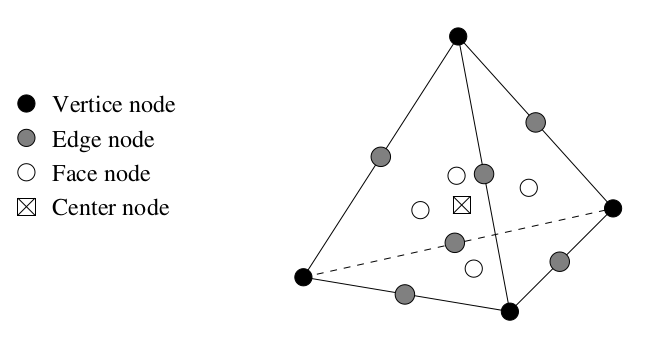
\includegraphics[width=9cm]{images/crouzeix-raviart/p2pp1_3D1}
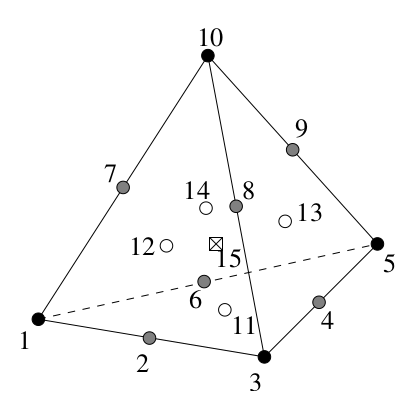
\includegraphics[width=5cm]{images/crouzeix-raviart/p2pp1_3D2}

The velocity shape functions are:
\begin{eqnarray}
\phi_i &=& \lambda_i(2\lambda_i-1) + 3 (\lambda_i\lambda_j \lambda_k + \lambda_i\lambda_j\lambda_l + \lambda_i\lambda_k\lambda_l) -4 \lambda_i\lambda_j\lambda_k\lambda_l \\
\phi_{ij} &=& 4\lambda_i\lambda_j - 12( \lambda_i\lambda_j\lambda_k+\lambda_i\lambda_j\lambda_l  ) +32 \lambda_i\lambda_j\lambda_k \lambda_l \\
\phi_{ijk} &=& 27  \lambda_i\lambda_j\lambda_k - 108 \lambda_i\lambda_j\lambda_k \lambda_l \\
\phi_c &=& 256 \lambda_i\lambda_j\lambda_k\lambda_l
\end{eqnarray}

\todo[inline]{REFS ??? better definition of functions !}

%.....................................................................
\subsubsection{Linear basis functions for tetrahedra ($P_1$)}
\index{general}{$P_1$}

This is essentially in the $Q_2\times P_{-1}$ element. 

I choose the reduced coordinates of the pressure nodes to be :

\begin{tabular}{cccc}
\hline
point & r & s & t \\
\hline
1& 1/2 &-1/2 &-1/2\\
2& -1/2 &1/2 &-1/2\\
3& -1/2 &-1/2& 1/2\\
4& 1/2 &1/2& 1/2 \\
\hline
\end{tabular}

Inside the element the pressure is given as a linear function of the reduced coordinates $r,s,t$:
\[
p(r,s,t)=a+br+cs+dt
\]
This expression must exactly interpolate the pressure at all four pressure nodes:
\begin{eqnarray}
p_1 
&=& p(r_1,s_1,t_1) 
= a+br_1+cs_1+dt_1 
= a+b/2-c/2-d/2\nonumber\\
p_2
&=& p(r_2,s_2,t_2)
= a+br_2+cs_2+dt_2
= a-b/2+c/2-d/2\nonumber\\
p_3
&=& p(r_3,s_3,t_3) 
= a+br_3+cs_3+dt_3 
= a-b/2-c/2+d/2\nonumber\\
p_4
&=& p(r_4,s_4,t_4) 
= a+br_4+cs_4+dt_4
= a+b/2+c/2+d/2\nonumber
\end{eqnarray}
or,
\begin{equation}
\left(
\begin{array}{cccc}
1 & 1/2 & -1/2 & -1/2 \\
1 & -1/2 & +1/2 & -1/2 \\
1 & -1/2 & -1/2 & +1/2 \\
1 & 1/2 & +1/2 & +1/2 
\end{array}
\right)
\left(
\begin{array}{c}
a\\b\\c\\d
\end{array}
\right)=
\left(
\begin{array}{c}
p_1\\p_2\\p_3\\p_4
\end{array}
\right)
\nonumber
\end{equation}

The matrix is invertible and we get:
\[
\left(
\begin{array}{c}
a\\b\\c\\d
\end{array}
\right)=
\left(
\begin{array}{cccc}
1/4 & 1/4 & 1/4 & 1/4 \\
1/2 & -1/2 & -1/2 & 1/2 \\
-1/2 & 1/2 & -1/2 & 1/2 \\
-1/2 & -1/2 & 1/2 & 1/2
\end{array}
\right)
\left(
\begin{array}{c}
p_1\\p_2\\p_3\\p_4
\end{array}
\right)
\]

so 
\begin{eqnarray}
p(r,s,t)
&=& a+br+cs+dt \nonumber\\
&=& \frac{1}{4}(p_1+p_2+p_3+p_4)
+\frac{1}{2}(p_1-p_2-p_3+p_4)r
+\frac{1}{2}(-p_1+p_2-p_3+p_4)s
+\frac{1}{2}(-p_1-p_2+p_3+p_4)t\nonumber\\
&=&
\frac{1}{4}(1+2r-2s-2t)p_1+
\frac{1}{4}(1-2r+2s-2t)p_2+
\frac{1}{4}(1-2r-2s+2t)p_3+
\frac{1}{4}(1+2r+2s+2t)p_4 \nonumber\\
&=& \sum_{i=1}^4 N_i(r,s,t) p_i
\end{eqnarray}
with
\begin{eqnarray}
N_1(r,s,t) &=& \frac{1}{4}(1+2r-2s-2t)\nonumber\\
N_2(r,s,t) &=& \frac{1}{4}(1-2r+2s-2t)\nonumber\\
N_3(r,s,t) &=& \frac{1}{4}(1-2r-2s+2t)\nonumber\\
N_4(r,s,t) &=& \frac{1}{4}(1+2r+2s+2t)\nonumber
\end{eqnarray}

%%%%%%%%%%%%%%%%%%%%%%%%%%%%%%%%%%%%%%%%%%%%%%%%%%%%%%%%%%%%%%%%%%%%%
\subsubsection{20-node serendipity basis functions in 3D ($Q_2^{(20)}$)}
\index{general}{$Q_2^{(20)}$} \index{general}{Serendipity element}

The serendipity elements are those rectangular elements which have no
interior nodes \cite[p91]{reddybook2}.

\begin{verbatim}
   t
   |
   .--s
  /
 r
                                    05=====20=====08 
                                    |             |  
                                    |             |  
                  17 - - - - - -19  13            16
                  .              .  |             |  
                  .              .  |             |  
06=====18=====07  .              .  01=====12=====04 @ r=-1
|             |   .              . 
|             |   .              .  
14            15  09 - - - - - -11 @ r=0
|             |   
|             |  
02=====10=====03 @ r=+1
\end{verbatim}

\todo[inline]{find/build shape functions!}


 %-------------------------------
\newpage
\subsection{Low order elements recap} Let us assume a Cartesian domain discretised in $nel_x \times nel_y$
elements in 2D and $nel_x \times nel_y \times nel_z$ elements in 3D.
Focusing only on the total number of velocity dofs (the values indicated after the 
arrows are the limits when $nel_x=nel_y=nel_z >> 1$):

\begin{itemize}

\item $Q_1 \times P_0$, $Q_1 \times Q_1$
\begin{eqnarray}
ndof_{2D}     &=&2 (nel_x+1) \cdot (nel_y+1) 
\qquad \rightarrow \qquad 2 \cdot nel_x^2   \nonumber\\
ndof_{3D}&=&3 (nel_x+1) \cdot (nel_y+1) \cdot (nel_z+1)
\qquad \rightarrow \qquad 3 \cdot nel_x^3 \nonumber
\end{eqnarray}

\item $Q_2 \times P_{-1}$, $Q_2 \times Q_1$
\begin{eqnarray}
ndof_{2D}      &=&2 (2nel_x+1) \cdot (2nel_y+1) 
\qquad \rightarrow \qquad 8 \cdot nel_x^2   \nonumber\\
ndof_{3D}&=&3 (2nel_x+1) \cdot (2nel_y+1) \cdot (2nel_z+1)
\qquad \rightarrow \qquad 24 \cdot nel_x^3 \nonumber
\end{eqnarray}


\item $Q_1^+ \times P_0$

\begin{eqnarray}
ndof_{2D}     &=&2 (nel_x+1) \cdot (nel_y+1) + (nel_x+1)\cdot nel_y + nel_x\cdot(nel_y+1)
\qquad \rightarrow \qquad 4 \cdot nel_x^2   \nonumber\\
ndof_{3D}&=&3 (nel_x+1) \cdot (nel_y+1) \cdot (nel_z+1) \nonumber\\
&+&  (nel_x+1)\cdot nel_y \cdot nel_z + nelx\cdot (nel_y+1) \cdot nelz + nelx\cdot nely \cdot (nel_z+1)
\quad \rightarrow \quad 6 \cdot nel_x^3 \nonumber
\end{eqnarray}

\item $Q_1 \times Q_1$+1 bubble

\begin{eqnarray}
ndof_{2D}&=& 2[(nel_x+1) \cdot (nel_y+1)  + \cdot nelx\cdot nely ]
\quad \rightarrow \quad 4 \cdot nel_x^2 \nonumber
\end{eqnarray}

%\item $Q_1^+ \times Q_1$
%\begin{eqnarray}
%ndof_{2D}  &=&2 [ (nel_x+1) \cdot (nel_y+1) + nel_x \cdot nel_y ]
%\qquad \rightarrow \qquad 4 \cdot nel_x^2   \nonumber
%ndof_{3D}  &=&3 [ (nel_x+1) \cdot (nel_y+1) \cdot (nel_z+1) + nel_x \cdot nel_y \cdot nel_z ]
%\qquad \rightarrow \qquad 6 \cdot nel_x^3 \nonumber
%\end{eqnarray}

\item $Q_1 \times Q_1$+2 bubbles

\begin{eqnarray}
ndof_{3D}&=& 3[(nel_x+1) \cdot (nel_y+1) \cdot  (nel_z+1) + 2\cdot nelx\cdot nely \cdot nelz]
\quad \rightarrow \quad 9 \cdot nel_x^3 \nonumber
\end{eqnarray}


\item Rannacher-turek or DSSY:

\begin{eqnarray}
ndof_{2D}&=& 2[(nel_y+1) \cdot nel_x+nel_y\cdot(nel_x+1)  ] 
\quad\rightarrow \quad 4 \cdot nel_x^2 \nonumber\nn\\
ndof_{3D}&=& 3[ nel_x\cdot (nel_y+1)\cdot nel_z + (nel_x+1) \cdot nel_y\cdot nel_z  +nel_x\cdot nel_y\cdot (nel_z+1) ]  
\quad \rightarrow \quad 9 \cdot nel_x^3 \nonumber
\end{eqnarray}
 

\end{itemize}


If we now assume $nel_x=nel_y=nel_z$, we can then plot the values above as a function of $nel_x$:
\begin{center}
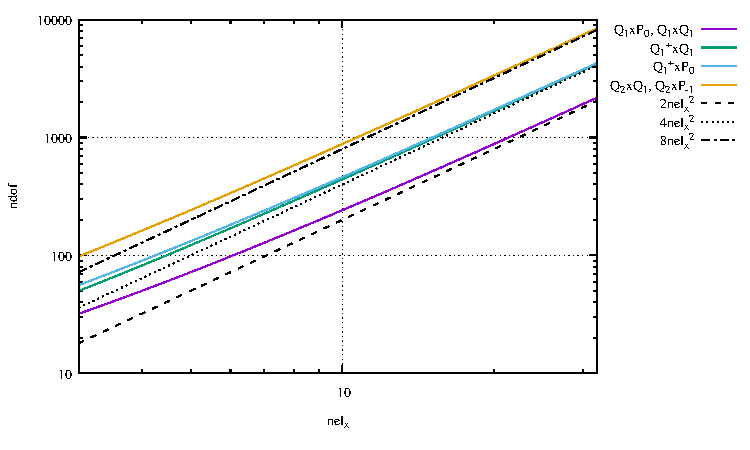
\includegraphics[width=7.5cm]{images/elements/ndof2D.pdf}
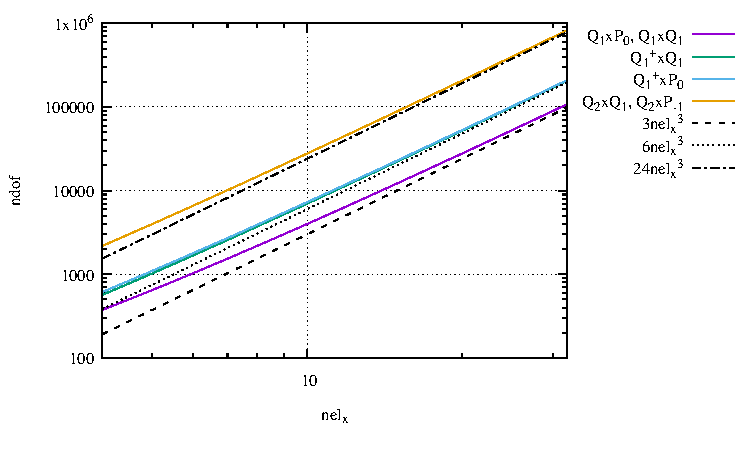
\includegraphics[width=7.5cm]{images/elements/ndof3D.pdf}
\end{center}

We see that the $Q_1^+\times Q_1$ and $Q_1^+ \times P_0$ actually 
ield the same number of velocity dofs. 

Simply based on the dof count and wishing for a (bi/tri)linear approximation 
for pressure, we must conclude that the $Q_1\times Q_1$+2 bubbles is the most desirable 
since it is also LBB stable.

\begin{center}
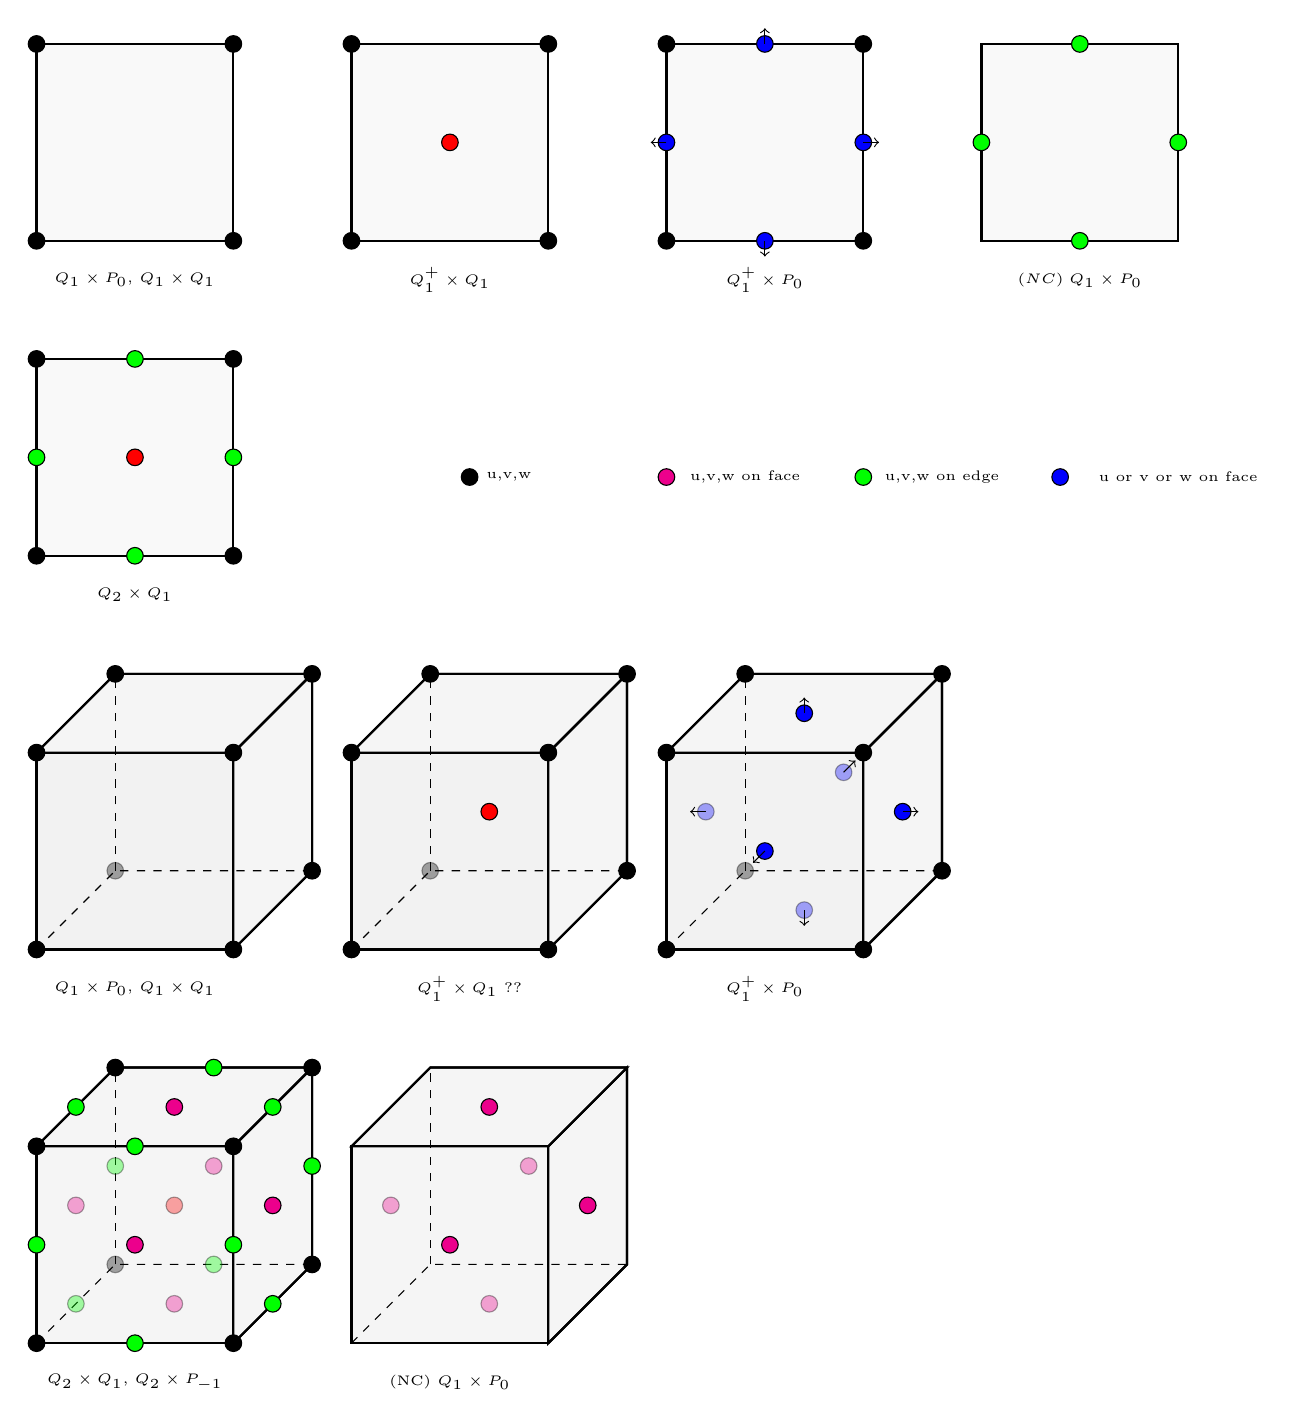
\begin{tikzpicture}
%\draw[fill=gray!23,gray!23](0,0) rectangle (20,10);
%\draw[step=0.5cm,gray,very thin] (0,0) grid (18,18); %background grid

%%%%%%%%%%%%%%%%%%%%%%%%%%%%%%%%%%%%%%%%%%%%%%%%%%%%%%%%%%%%%%%%%%%%
%bottom row
%%%%%%%%%%%%%%%%%%%%%%%%%%%%%%%%%%%%%%%%%%%%%%%%%%%%%%%%%%%%%%%%%%%%
\draw[thick,fill=gray!8] (1,1) -- (3.5,1) -- (3.5,3.5) -- (1,3.5) -- cycle;
\draw[thick,fill=gray!8] (5,1) -- (7.5,1) -- (7.5,3.5) -- (5,3.5) -- cycle;
%\draw[thick,fill=gray!8] (9,1) -- (11.5,1) -- (11.5,3.5) -- (9,3.5) -- cycle;
%\draw[thick,fill=gray!8] (13,1) -- (15.5,1) -- (15.5,3.5) -- (13,3.5) -- cycle;

%right sides
\draw[thick,fill=gray!8] (3.5,1) -- (4.5,2) -- (4.5,4.5) -- (3.5,3.5) -- cycle;
\draw[thick,fill=gray!8] (7.5,1) -- (8.5,2) -- (8.5,4.5) -- (7.5,3.5) -- cycle;
%\draw[thick,fill=gray!8] (11.5,1) -- (12.5,2) -- (12.5,4.5) -- (11.5,3.5) -- cycle;
%\draw[thick,fill=gray!8] (15.5,1) -- (16.5,2) -- (16.5,4.5) -- (15.5,3.5) -- cycle;

%tops
\draw[thick,fill=gray!8] (1,3.5) -- (3.5,3.5) -- (4.5,4.5) -- (2,4.5) -- cycle;
\draw[thick,fill=gray!8] (5,3.5) -- (7.5,3.5) -- (8.5,4.5) -- (6,4.5) -- cycle;
%\draw[thick,fill=gray!8] (9,3.5) -- (11.5,3.5) -- (12.5,4.5) -- (10,4.5) -- cycle;
%\draw[thick,fill=gray!8] (13,3.5) -- (15.5,3.5) -- (16.5,4.5) -- (14,4.5) -- cycle;

\draw[thick] (1,3.5) -- (2,4.5) -- (4.5,4.5) -- (4.5,2) -- (3.5,1);
\draw[thick] (5,3.5) -- (6,4.5) -- (8.5,4.5) -- (8.5,2) -- (7.5,1);
%\draw[thick] (9,3.5) -- (10,4.5) -- (12.5,4.5) -- (12.5,2) -- (11.5,1);
%\draw[thick] (13,3.5) -- (14,4.5) -- (16.5,4.5) -- (16.5,2) -- (15.5,1);

\draw[thick] (3.5,3.5) -- (4.5,4.5) ;
\draw[thick] (7.5,3.5) -- (8.5,4.5) ;
%\draw[thick] (11.5,3.5) -- (12.5,4.5) ;
%\draw[thick] (15.5,3.5) -- (16.5,4.5) ;

\draw[dashed] (1,1) -- (2,2) -- (4.5,2) ;\draw[dashed] (2,2) -- (2,4.5);
\draw[dashed] (5,1) -- (6,2) -- (8.5,2) ;\draw[dashed] (6,2) -- (6,4.5);
%\draw[dashed] (9,1) -- (10,2) -- (12.5,2) ;\draw[dashed] (10,2) -- (10,4.5);
%\draw[dashed] (13,1) -- (14,2) -- (16.5,2) ;\draw[dashed] (14,2)--(14,4.5);

\draw[black,fill=black] (1,1)   circle (3pt);
\draw[black,fill=black] (3.5,1)   circle (3pt);
\draw[black,fill=black] (3.5,3.5)   circle (3pt);
\draw[black,fill=black] (1,3.5)   circle (3pt);
\draw[black,fill=black] (2,4.5)   circle (3pt);
\draw[black,fill=black] (4.5,4.5)   circle (3pt);
\draw[black,fill=black] (4.5,2)   circle (3pt);
\draw[black,fill=black,opacity=0.35] (2,2)   circle (3pt);

%\draw[black,fill=black] (5,1)   circle (3pt);
%\draw[black,fill=black] (7.5,1)   circle (3pt);
%\draw[black,fill=black] (7.5,3.5)   circle (3pt);
%\draw[black,fill=black] (5,3.5)   circle (3pt);
%\draw[black,fill=black] (6,4.5)   circle (3pt);
%\draw[black,fill=black] (8.5,4.5)   circle (3pt);
%\draw[black,fill=black] (8.5,2)   circle (3pt);
%\draw[black,fill=black,opacity=0.35] (6,2)   circle (3pt);

%\draw[black,fill=black] (9,1)   circle (3pt);
%\draw[black,fill=black] (11.5,1)   circle (3pt);
%\draw[black,fill=black] (11.5,3.5)   circle (3pt);
%\draw[black,fill=black] (9,3.5)   circle (3pt);
%\draw[black,fill=black] (10,4.5)   circle (3pt);
%\draw[black,fill=black] (12.5,4.5)   circle (3pt);
%\draw[black,fill=black] (12.5,2)   circle (3pt);
%\draw[black,fill=black,opacity=0.35] (10,2)   circle (3pt);

%\draw[black,fill=black] (13,1)   circle (3pt);
%\draw[black,fill=black] (15.5,1)   circle (3pt);
%\draw[black,fill=black] (15.5,3.5)   circle (3pt);
%\draw[black,fill=black] (13,3.5)   circle (3pt);
%\draw[black,fill=black] (14,4.5)   circle (3pt);
%\draw[black,fill=black] (16.5,4.5)   circle (3pt);
%\draw[black,fill=black] (16.5,2)   circle (3pt);
%\draw[black,fill=black,opacity=0.35] (14,2)   circle (3pt);


%%%%%%%%%%%%%%%%%%%%%%%%%%%%%%%%%%%%%%%%%%%%%%%%%%%%%%%%%%%%%%%%%%%%
%3rd row 
%%%%%%%%%%%%%%%%%%%%%%%%%%%%%%%%%%%%%%%%%%%%%%%%%%%%%%%%%%%%%%%%%%%%

\draw[thick,fill=gray!5] (1,15) -- (3.5,15) -- (3.5,17.5) -- (1,17.5) -- cycle;
\draw[thick,fill=gray!5] (5,15) -- (7.5,15) -- (7.5,17.5) -- (5,17.5) -- cycle;
\draw[thick,fill=gray!5] (9,15) -- (11.5,15) -- (11.5,17.5) -- (9,17.5) -- cycle;
\draw[thick,fill=gray!5] (13,15) -- (15.5,15) -- (15.5,17.5) -- (13,17.5) -- cycle;

\draw[black,fill=black] (1,15)   circle (3pt);
\draw[black,fill=black] (3.5,15)   circle (3pt);
\draw[black,fill=black] (1,17.5)   circle (3pt);
\draw[black,fill=black] (3.5,17.5)   circle (3pt);
\node[] at (2.25,14.5) {\tiny $Q_1\times P_0$, $Q_1\times Q_1$};


\draw[black,fill=black] (5,15)   circle (3pt);
\draw[black,fill=black] (7.5,15)   circle (3pt);
\draw[black,fill=black] (5,17.5)   circle (3pt);
\draw[black,fill=black] (7.5,17.5)   circle (3pt);
\node[] at (6.25,14.5) {\tiny $Q_1^+\times Q_1$};
\draw[black,fill=red] (6.25,16.25)   circle (3pt);

\draw[black,fill=black] (9,15)   circle (3pt);
\draw[black,fill=black] (11.5,15)   circle (3pt);
\draw[black,fill=black] (9,17.5)   circle (3pt);
\draw[black,fill=black] (11.5,17.5)   circle (3pt);
\node[] at (10.25,14.5) {\tiny $Q_1^+\times P_0$};

\draw[black,fill=blue] (9,16.25)   circle (3pt);
\draw[black,fill=blue] (11.5,16.25)   circle (3pt);
\draw[black,fill=blue] (10.25,15)   circle (3pt);
\draw[black,fill=blue] (10.25,17.5)   circle (3pt);

\draw[fill=blue,->] (9,16.25) -- (8.8,16.25); 
\draw[fill=blue,->] (11.5,16.25) -- (11.7,16.25); 
\draw[fill=blue,->] (10.25,15) -- (10.25,14.8); 
\draw[fill=blue,->] (10.25,17.5) -- (10.25,17.7); 


\draw[black,fill=green] (14.25,15)   circle (3pt);
\draw[black,fill=green] (14.25,17.5)   circle (3pt);
\draw[black,fill=green] (13,16.25)   circle (3pt);
\draw[black,fill=green] (15.5,16.25)   circle (3pt);
\node[] at (14.25,14.5) {\tiny $(NC)\; Q_1\times P_0$};

%%%%%%%%%%%%%%%%%%%%%%%%%%%%%%%%%%%%%%%%%%%%%%%%%%%%%%%%%%%%%%%%%%%%
%2nd row 
%%%%%%%%%%%%%%%%%%%%%%%%%%%%%%%%%%%%%%%%%%%%%%%%%%%%%%%%%%%%%%%%%%%%

\draw[thick,fill=gray!5] (1,11) -- (3.5,11) -- (3.5,13.5) -- (1,13.5) -- cycle;
%\draw[thick,fill=gray!5] (5,11) -- (7.5,11) -- (7.5,13.5) -- (5,13.5) -- cycle;
%\draw[thick,fill=gray!5] (9,11) -- (11.5,11) -- (11.5,13.5) -- (9,13.5) -- cycle;
%\draw[thick,fill=gray!5] (13,11) -- (15.5,11) -- (15.5,13.5) -- (13,13.5) -- cycle;

\draw[black,fill=black] (1,11)   circle (3pt);
\draw[black,fill=green] (2.25,11)   circle (3pt);
\draw[black,fill=black] (3.5,11)   circle (3pt);
\draw[black,fill=green] (1,12.25)   circle (3pt);
\draw[black,fill=red] (2.25,12.25)   circle (3pt);
\draw[black,fill=green] (3.5,12.25)   circle (3pt);
\draw[black,fill=black] (1,13.5)   circle (3pt);
\draw[black,fill=green] (2.25,13.5)   circle (3pt);
\draw[black,fill=black] (3.5,13.5)   circle (3pt);
\node[] at (2.25,10.5) {\tiny $Q_2\times Q_1$};



%%%%%%%%%%%%%%%%%%%%%%%%%%%%%%%%%%%%%%%%%%%%%%%%%%%%%%%%%%%%%%%%%%%%
%1st row 
%%%%%%%%%%%%%%%%%%%%%%%%%%%%%%%%%%%%%%%%%%%%%%%%%%%%%%%%%%%%%%%%%%%%
\draw[thick,fill=gray!10] (1,6) -- (3.5,6) -- (3.5,8.5) -- (1,8.5) -- cycle;
\draw[thick,fill=gray!10] (5,6) -- (7.5,6) -- (7.5,8.5) -- (5,8.5) -- cycle;
\draw[thick,fill=gray!10] (9,6) -- (11.5,6) -- (11.5,8.5) -- (9,8.5) -- cycle;
%\draw[thick,fill=gray!10] (13,6) -- (15.5,6) -- (15.5,8.5) -- (13,8.5) -- cycle;

%right sides
\draw[thick,fill=gray!8] (3.5,6) -- (4.5,7) -- (4.5,9.5) -- (3.5,8.5) -- cycle;
\draw[thick,fill=gray!8] (7.5,6) -- (8.5,7) -- (8.5,9.5) -- (7.5,8.5) -- cycle;
\draw[thick,fill=gray!8] (11.5,6) -- (12.5,7) -- (12.5,9.5) -- (11.5,8.5) -- cycle;
%\draw[thick,fill=gray!8] (15.5,6) -- (16.5,7) -- (16.5,9.5) -- (15.5,8.5) -- cycle;

%tops
\draw[thick,fill=gray!8] (1,8.5) -- (3.5,8.5) -- (4.5,9.5) -- (2,9.5) -- cycle;
\draw[thick,fill=gray!8] (5,8.5) -- (7.5,8.5) -- (8.5,9.5) -- (6,9.5) -- cycle;
\draw[thick,fill=gray!8] (9,8.5) -- (11.5,8.5) -- (12.5,9.5) -- (10,9.5) -- cycle;
%\draw[thick,fill=gray!8] (13,8.5) -- (15.5,8.5) -- (16.5,9.5) -- (14,9.5) -- cycle;


\draw[thick] (1,8.5) -- (2,9.5) -- (4.5,9.5) -- (4.5,7) -- (3.5,6);
\draw[thick] (5,8.5) -- (6,9.5) -- (8.5,9.5) -- (8.5,7) -- (7.5,6);
\draw[thick] (9,8.5) -- (10,9.5) -- (12.5,9.5) -- (12.5,7) -- (11.5,6);
%\draw[thick] (13,8.5) -- (14,9.5) -- (16.5,9.5) -- (16.5,7) -- (15.5,6);

\draw[thick] (3.5,8.5) -- (4.5,9.5) ;
\draw[thick] (7.5,8.5) -- (8.5,9.5) ;
\draw[thick] (11.5,8.5) -- (12.5,9.5) ;
%\draw[thick] (15.5,8.5) -- (16.5,9.5) ;

\draw[dashed] (1,6) -- (2,7) -- (4.5,7)    ;\draw[dashed] (2,7) -- (2,9.5);
\draw[dashed] (5,6) -- (6,7) -- (8.5,7)    ;\draw[dashed] (6,7) -- (6,9.5);
\draw[dashed] (9,6) -- (10,7) -- (12.5,7)  ;\draw[dashed] (10,7) -- (10,9.5);
%\draw[dashed] (13,6) -- (14,7) -- (16.5,7) ;\draw[dashed] (14,7) -- (14,9.5);

\draw[black,fill=black] (1,6)   circle (3pt);
\draw[black,fill=black] (3.5,6)   circle (3pt);
\draw[black,fill=black] (3.5,8.5)   circle (3pt);
\draw[black,fill=black] (1,8.5)   circle (3pt);
\draw[black,fill=black] (2,9.5)   circle (3pt);
\draw[black,fill=black] (4.5,9.5)   circle (3pt);
\draw[black,fill=black] (4.5,7)   circle (3pt);
\draw[black,fill=black,opacity=0.35] (2,7)   circle (3pt);

\draw[black,fill=black] (5,6)   circle (3pt);
\draw[black,fill=black] (7.5,6)   circle (3pt);
\draw[black,fill=black] (7.5,8.5)   circle (3pt);
\draw[black,fill=black] (5,8.5)   circle (3pt);
\draw[black,fill=black] (6,9.5)   circle (3pt);
\draw[black,fill=black] (8.5,9.5)   circle (3pt);
\draw[black,fill=black] (8.5,7)   circle (3pt);
\draw[black,fill=black,opacity=0.35] (6,7)   circle (3pt);

\draw[black,fill=black] (9,6)   circle (3pt);
\draw[black,fill=black] (11.5,6)   circle (3pt);
\draw[black,fill=black] (11.5,8.5)   circle (3pt);
\draw[black,fill=black] (9,8.5)   circle (3pt);
\draw[black,fill=black] (10,9.5)   circle (3pt);
\draw[black,fill=black] (12.5,9.5)   circle (3pt);
\draw[black,fill=black] (12.5,7)   circle (3pt);
\draw[black,fill=black,opacity=0.35] (10,7)   circle (3pt);

%\draw[black,fill=black] (13,5)   circle (2pt);
%\draw[black,fill=black] (15.5,5)   circle (2pt);
%\draw[black,fill=black] (15.5,7.5)   circle (2pt);
%\draw[black,fill=black] (13,7.5)   circle (2pt);
%\draw[black,fill=black] (14,8.5)   circle (2pt);
%\draw[black,fill=black] (16.5,8.5)   circle (2pt);
%\draw[black,fill=black] (16.5,6)   circle (2pt);
%\draw[black,fill=black,opacity=0.35] (14,6)   circle (2pt);


\node[] at (2.25,5.5) {\tiny $Q_1\times P_0$, $Q_1\times Q_1$};


\node[] at (6.5,5.5) {\tiny $Q_1^+\times Q_1$ ??};
\draw[black,fill=red] (6.75,7.75)   circle (3pt);

\node[] at (10.25,5.5) {\tiny $Q_1^+\times P_0$};
\draw[black,fill=blue,opacity=0.35] (9.5,7.75)   circle (3pt);
\draw[black,fill=blue] (12,7.75)   circle (3pt);
\draw[black,fill=blue,opacity=0.35] (10.75,6.5)   circle (3pt);
\draw[black,fill=blue] (10.75,9)   circle (3pt);
\draw[black,fill=blue] (10.25,7.25)   circle (3pt);
\draw[black,fill=blue,opacity=0.35] (11.25,8.25)   circle (3pt);

\draw[fill=blue,->] (9.5,7.75) -- (9.3,7.75); 
\draw[fill=blue,->] (12,7.75) -- (12.2,7.75); 
\draw[fill=blue,->] (10.75,6.5) -- (10.75,6.3); 
\draw[fill=blue,->] (10.75,9) -- (10.75,9.2); 
\draw[fill=blue,->] (10.25,7.25)  -- (10.1,7.1) ;
\draw[fill=blue,->] (11.25,8.25)  -- (11.4,8.4) ;

\node[] at (2.25,0.5) {\tiny $Q_2\times Q_1$, $Q_2\times P_{-1}$};

\draw[black,fill=red,opacity=0.35] (2.75,2.75)   circle (3pt);

\draw[black,fill=magenta,opacity=0.35] (1.5,2.75)   circle (3pt);
\draw[black,fill=magenta] (4,2.75)   circle (3pt);
\draw[black,fill=magenta,opacity=0.35] (2.75,1.5)   circle (3pt);
\draw[black,fill=magenta] (2.75,4)   circle (3pt);
\draw[black,fill=magenta] (2.25,2.25)   circle (3pt);
\draw[black,fill=magenta,opacity=0.35] (3.25,3.25)   circle (3pt);

\draw[black,fill=green] (1,2.25)   circle (3pt);
\draw[black,fill=green] (3.5,2.25)   circle (3pt);
\draw[black,fill=green,opacity=0.35] (2,3.25)   circle (3pt);
\draw[black,fill=green] (4.5,3.25)   circle (3pt);
\draw[black,fill=green,opacity=0.35] (1.5,1.5)   circle (3pt);
\draw[black,fill=green] (4,1.5)   circle (3pt);
\draw[black,fill=green] (2.25,1)   circle (3pt);
\draw[black,fill=green,opacity=0.35] (3.25,2)   circle (3pt);
\draw[black,fill=green] (1.5,4)   circle (3pt);
\draw[black,fill=green] (4,4)   circle (3pt);
\draw[black,fill=green] (2.25,3.5)   circle (3pt);
\draw[black,fill=green] (3.25,4.5)   circle (3pt);

\node[] at (6.25,0.5) {\tiny (NC) $Q_1\times P_0$};
\draw[black,fill=magenta,opacity=0.35] (5.5,2.75)   circle (3pt);
\draw[black,fill=magenta] (8,2.75)   circle (3pt);
\draw[black,fill=magenta,opacity=0.35] (6.75,1.5)   circle (3pt);
\draw[black,fill=magenta] (6.75,4)   circle (3pt);
\draw[black,fill=magenta] (6.25,2.25)   circle (3pt);
\draw[black,fill=magenta,opacity=0.35] (7.25,3.25)   circle (3pt);

\draw[black,fill=black]   (6.5,12) circle (3pt); \node[] at (7,12) {\tiny u,v,w};
\draw[black,fill=magenta] (9,12) circle (3pt); \node[] at (10,12) {\tiny u,v,w on face};
\draw[black,fill=green] (11.5,12) circle (3pt); \node[] at (12.5,12) {\tiny u,v,w on edge};
\draw[black,fill=blue] (14,12) circle (3pt); \node[] at (15.5,12) {\tiny u or v or w on face};

%\draw[black,fill=blue] (1,3.5) circle (2pt); \node[] at (1,3.7) {\tiny \color{blue} 60};

%\draw[black,fill=green](14.75,4.75) circle (2pt);\node[] at (14.75,4.95){\tiny\color{green}121};

%\draw[black,fill=red] (6.25,4.75) circle (2pt); \node[] at (6.25,4.95) {\tiny \color{red} 148};

%\node[] at (1.5,2.75) {\tiny \color{magenta} (0)};


%\draw[thick,->] (0,3) -- (0,4); %x
%\draw[thick,->] (0,3) -- (1,2.5); %y
%\node[] at (1,2.125) {$y$};
%\node[] at (0.25,4) {$z$};

\end{tikzpicture}
\end{center}

Add DSSY, RT, Q1Q1+2 bubbles

\vspace{.5cm}

\begin{tabular}{llll}
\hline
2D &  \\ 
Rannacher-Turek & NCQ1P0 & \stone 77 & pb with buoyancy-driven flow \\
Lamichhane      & Q1+Q1  & \stone 72, \stone 74  & \\ 
DSSY            &        & \stone 77  pb with buoyancy-driven flow \\
Fortin          &        & \stone 80 \\
\hline
\hline
3D & \\
Rannacher-Turek & NCQ1P0  & \elefant &  \\
Lamichhane      & Q1+Q1   & \stone  & Does not work \\ 
DSSY & \\
Fortin & & \stone 81 \\
\hline
\end{tabular}
 %-------------------------------------
\newpage
\subsection{On the meaning of basis functions} \begin{flushright} {\tiny {\color{gray} basis\_functions\_meaning.tex.tex}} \end{flushright}
%~~~~~~~~~~~~~~~~~~~~~~~~~~~~~~~~~~~~~~~~~~~~~~~~~~~~~~~~~~~~~~~~~~~~~~~~~~~~~~~~~~~~~~~~~~~~~~~~~~


\subsubsection{In one dimension}

Let us consider a 1D domain subdivided in 3 elements. We then consider the four linear basis functions 
attached to each node. On the following sketch these are not depicted on a single element with 
reduced coordinates but instead for the whole domain in the natural coordinate $x$:

\begin{flushright} {\tiny {\color{gray} (tikz\_basisfunctions.tex)}} \end{flushright}
%~~~~~~~~~~~~~~~~~~~~~~~~~~~~~~~~~~~~~~~~~~~~~~~~~~~~~~~~~~~~~~~~~~~~~~~~~~~~~~~~~~~~~~~~~~~~~~~~~~

\begin{center}
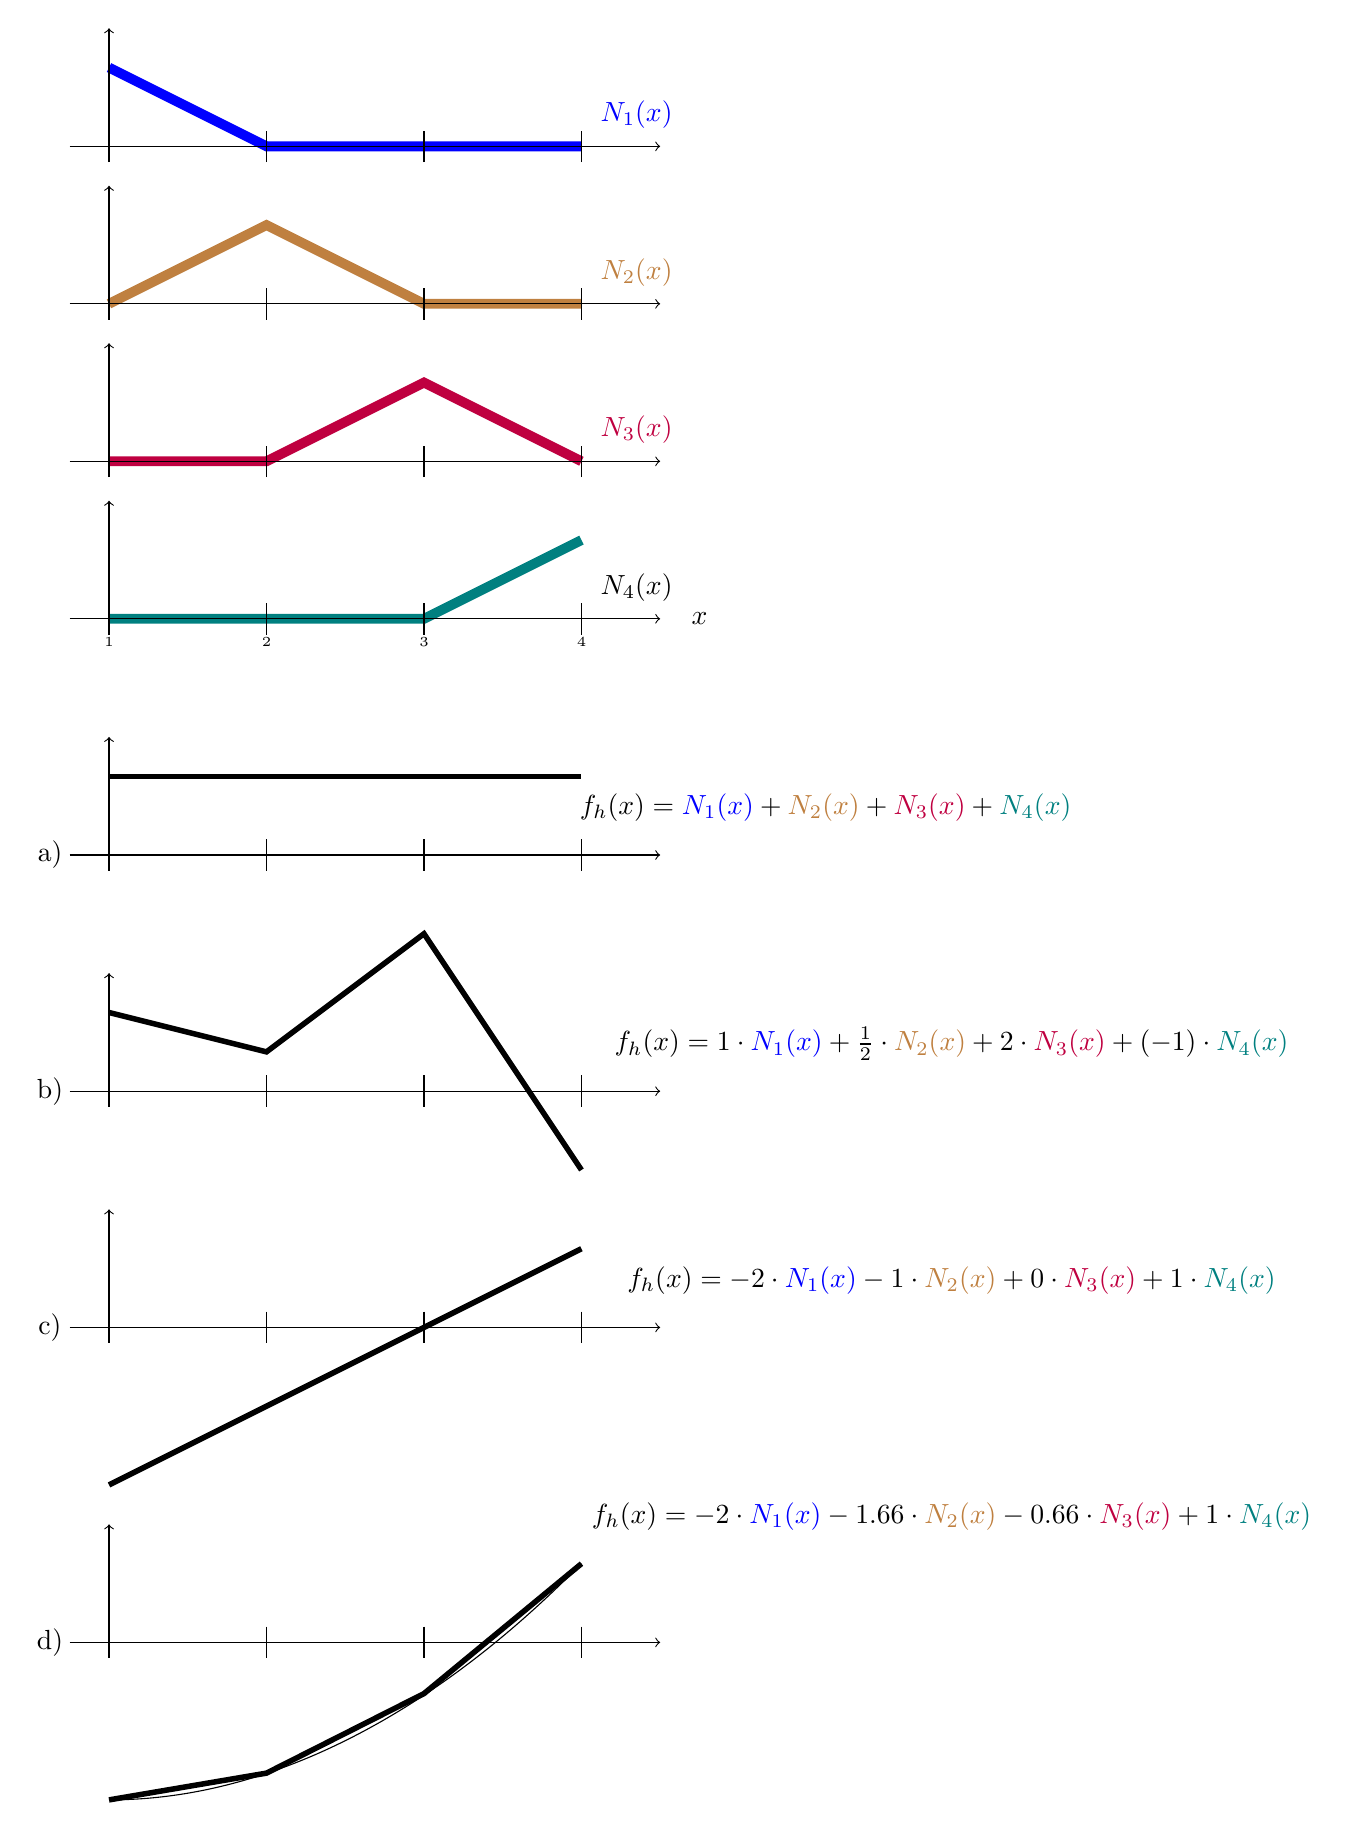
\begin{tikzpicture}
%\draw[step=0.5cm,gray,very thin] (0,-15) grid (15,10); 

%N1
\node[] at (7.7,7.4) {\color{blue}$N_1(x)$};
\draw[line width=1.25mm,color=blue] (1,8)--(3,7)--(5,7)--(7,7);
\draw [->] (0.5,7) -- (8,7);
\draw [->] (1,7) -- (1,8.5);
\draw [-] (1,6.8) -- (1,7.2);
\draw [-] (3,6.8) -- (3,7.2);
\draw [-] (5,6.8) -- (5,7.2);
\draw [-] (7,6.8) -- (7,7.2);

%N2
\node[] at (7.7,5.4) {\color{brown} $N_2(x)$};
\draw[line width=1.25mm,color=brown] (1,5)--(3,6)--(5,5)--(7,5);
\draw [->] (0.5,5) -- (8,5);
\draw [->] (1,5) -- (1,6.5);
\draw [-] (1,4.8) -- (1,5.2);
\draw [-] (3,4.8) -- (3,5.2);
\draw [-] (5,4.8) -- (5,5.2);
\draw [-] (7,4.8) -- (7,5.2);

%N3
\node[] at (7.7,3.4) {\color{purple}$N_3(x)$};
\draw[line width=1.25mm,color=purple] (1,3)--(3,3)--(5,4)--(7,3);
\draw [->] (0.5,3) -- (8,3);
\draw [->] (1,3) -- (1,4.5);
\draw [-] (1,2.8) -- (1,3.2);
\draw [-] (3,2.8) -- (3,3.2);
\draw [-] (5,2.8) -- (5,3.2);
\draw [-] (7,2.8) -- (7,3.2);

%N4
\node[] at (7.7,1.4) {$N_4(x)$};
\draw[line width=1.25mm,color=teal] (1,1)--(5,1)--(7,2);
\draw [->] (0.5,1) -- (8,1);
\draw [->] (1,1) -- (1,2.5);
\draw [-] (1,0.8) -- (1,1.2);
\draw [-] (3,0.8) -- (3,1.2);
\draw [-] (5,0.8) -- (5,1.2);
\draw [-] (7,0.8) -- (7,1.2);
\node[] at (8.5,1) {$x$};
\node[] at (1,0.7) {\tiny $1$};
\node[] at (3,0.7) {\tiny $2$};
\node[] at (5,0.7) {\tiny $3$};
\node[] at (7,0.7) {\tiny $4$};

\node[] at (0.25,-2) {a)};
\node[] at (10.1,-1.4) {$f_h(x)={\color{blue}N_1(x)}+{\color{brown} N_2(x)}+{\color{purple}N_3(x)}+{\color{teal}N_4(x)}$};
\draw[line width=0.7mm] (1,-1)--(7,-1);
\draw [->] (0.5,-2) -- (8,-2);
\draw [->] (1,-2) -- (1,-0.5);
\draw [-] (1,-1.8) -- (1,-2.2);
\draw [-] (3,-1.8) -- (3,-2.2);
\draw [-] (5,-1.8) -- (5,-2.2);
\draw [-] (7,-1.8) -- (7,-2.2);

\node[] at (0.25,-5) {b)};
\node[] at (11.7,-4.4) {$f_h(x)=1\cdot {\color{blue}N_1(x)}+\frac12\cdot {\color{brown} N_2(x)}+2\cdot {\color{purple}N_3(x)}+(-1)\cdot {\color{teal}N_4(x)}$};
\draw [->] (0.5,-5) -- (8,-5);
\draw [->] (1,-5) -- (1,-3.5);
\draw [-] (1,-4.8) -- (1,-5.2);
\draw [-] (3,-4.8) -- (3,-5.2);
\draw [-] (5,-4.8) -- (5,-5.2);
\draw [-] (7,-4.8) -- (7,-5.2);
\draw[line width=0.7mm] (1,-4)--(3,-4.5)--(5,-3)--(7,-6);

\node[] at (0.25,-8) {c)};
\node[] at (11.7,-7.4) {$f_h(x)=-2\cdot {\color{blue}N_1(x)}-1\cdot {\color{brown} N_2(x)}+0\cdot {\color{purple}N_3(x)}+1\cdot {\color{teal}N_4(x)}$};
\draw [->] (0.5,-8) -- (8,-8);
\draw [->] (1,-8) -- (1,-6.5);
\draw [-] (1,-7.8) -- (1,-8.2);
\draw [-] (3,-7.8) -- (3,-8.2);
\draw [-] (5,-7.8) -- (5,-8.2);
\draw [-] (7,-7.8) -- (7,-8.2);
\draw[line width=0.7mm] (1,-10)--(3,-9)--(5,-8)--(7,-7);

\node[] at (0.25,-12) {d)};
\draw [->] (0.5,-12) -- (8,-12);
\draw [->] (1,-12) -- (1,-10.5);
\draw [-] (1,-11.8) -- (1,-12.2);
\draw [-] (3,-11.8) -- (3,-12.2);
\draw [-] (5,-11.8) -- (5,-12.2);
\draw [-] (7,-11.8) -- (7,-12.2);
\draw (1,-14) parabola (7,-11);
\draw[line width=0.7mm] (1,-14)--(3,-13.66)--(5,-12.65)--(7,-11);
\node[] at (11.7,-10.4) {$f_h(x)=-2\cdot {\color{blue}N_1(x)}-1.66\cdot {\color{brown} N_2(x)}-0.66\cdot {\color{purple}N_3(x)}+1\cdot {\color{teal}N_4(x)}$};


\end{tikzpicture}
\end{center}


The four cases a,b,c,d are examples of combinations of these basis functions:
\[
f_h(x)=\sum_{i=1}^4 N_i(x) f_i
\]
Where $f_i$ are the values associated to the four nodes. 
We assume that the distance $h$ between nodes is 1.

Example a) illustrates the fact that the sum of all basis functions must be strictly equal to one everywhere
in the domain. Failing to do so would mean that the basis functions cannot represent a constant field (see
Section~\ref{ss:q12d}). 

Example b) illustrates a somewhat random combination of the basis functions, yielding a broken line. 

Example c) illustrates the fact that these linear basis functions can exactly represent a
linear function. When $f(x)=x-2$, then $f_1=f(0)=-2$, $f_2=f(1)=-1$, $f_3=f(2)=0$ and $f_4=f(3)=+1$, 
then $f_h(x)$ is exactly $f(x)$ on the domain.

Example d) illustrates the fact that linear basis functions cannot represent a parabola. Smaller and 
smaller elements will do an increasingly better job and will get closer to the curve but a 
systematic error will subsist.  


Note that these drawings are trivial to produce since $N_i(x_j)=\delta_{ij}$ by definition, so that 
$f_h(x_j)=f_j$.

%........................................................................
\subsubsection{In two dimensions}



 %-------------------
